% relatorio_rahardjo2007.tex: a reproducao da Serie B de Rahardjo et al. (2007) no NeoPZ (Projects/Rahardjo2007). Figuras
% e tabelas: gera_dados.py, com os dados de ~/projects/runs/rahardjo2007; ./gera.sh refaz tudo.
\documentclass[11pt,a4paper]{article}
\usepackage[utf8]{inputenc}
\usepackage[T1]{fontenc}
\usepackage[brazil]{babel}
\usepackage{lmodern,amsmath,amssymb,booktabs,graphicx,geometry,caption,float,xcolor}
\usepackage[hidelinks]{hyperref}
\geometry{margin=2.3cm}
\captionsetup{font=small}
\emergencystretch=2em
\providecommand{\versao}{}
\newcommand{\afazer}[1]{\textcolor{red}{[A FAZER: #1]}}
\IfFileExists{numeros.tex}{\newcommand{\difMedia}{0{,}00}
\newcommand{\difMax}{0{,}02}
\newcommand{\nCasos}{28}
\newcommand{\catOk}{21}
\newcommand{\catTot}{21}
\newcommand{\cincoN}{231}
\newcommand{\cincoRms}{0{,}017}
\newcommand{\cincoMax}{0{,}05}
\newcommand{\cincoFrac}{91}
\newcommand{\nCampos}{6}
\newcommand{\nMalhasF}{3}
\newcommand{\custoMedio}{59}
\newcommand{\custoMin}{46}
\newcommand{\custoMax}{67}
\newcommand{\campanha}{67}
\newcommand{\nFeitos}{28}
\newcommand{\nTotal}{28}
}{}
\providecommand{\nFeitos}{0}\providecommand{\nTotal}{28}\providecommand{\difMedia}{--}\providecommand{\difMax}{--}
\providecommand{\nCasos}{0}\providecommand{\nCampos}{0}\providecommand{\nMalhasF}{0}\providecommand{\iFeitos}{0}
\providecommand{\nCamposI}{0}\providecommand{\nPerfis}{0}\providecommand{\durErro}{--}

\title{Reprodução de Rahardjo et al.\ (2007), Série B:\\ o FS de um talude homogêneo sob chuva,\\ com ar passivo e com
ar ativo\\ \large relatório das simulações (\texttt{Projects/Rahardjo2007})}
\author{Diogo Cecílio}
\date{\versao}

\begin{document}
\maketitle

\begin{abstract}
H.~Rahardjo, T.~H.~Ong, R.~B.~Rezaur e E.~C.~Leong (2007), \emph{Factors controlling instability of homogeneous soil
slopes under rainfall} (J.\ Geotech.\ Geoenviron.\ Eng.\ 133(12):1532--1543), calculam no SEEP/W e no SLOPE/W o fator de
segurança de um talude homogêneo de 10~m a 45° sob chuvas de 24~h, em três solos residuais de Singapura. Na Série B a
intensidade varia de $k_s/40$ a $10\,k_s$; dela saem a Fig.~5 (o FS ao longo de 48~h), as Figs.~6 e 7 (o FS mínimo
contra a intensidade e a sigmoide da Eq.~6) e a Tabela~5 (onde está o nível d'água no FS mínimo). Aqui a Série B inteira
(28 rodadas: as 21 da Tabela~2 e os 7 pontos que só aparecem nas Figs.~6 e 7) é calculada com o modelo (iii) do
NeoPZ: esqueleto rígido e ar passivo, só a percolação da água, como no SEEP/W, e o FS pelo SRM de hora em hora.
As \nFeitos{} rodadas reproduzem o artigo dentro do erro de leitura das figuras: os FS mínimos ficam a até \difMax{}
dos da Fig.~6; os \cincoN{} pontos da Fig.~5 ficam a até \cincoMax{}, \cincoFrac\,\% deles a até 0,03; as \catTot{}
categorias de nível d'água da Tabela~5 saem iguais; e a Eq.~6 ajustada aos nossos pontos fica com os parâmetros do
artigo.

As mesmas rodadas com o ar ativo (modelo (i)) mudam a forma da curva do FS mínimo contra a intensidade. Nas chuvas
médias, o ar comprimido entre a frente de umedecimento e o nível d'água levanta a poropressão com o solo ainda não
saturado, e o FS mínimo cai até \quedaCem{} ($f_{100,-6}$ a \quedaCemI~mm/h) e \quedaCinq{} ($f_{50,-5}$ a
\quedaCinqI~mm/h). Nas chuvas fortes,
o ar preso não deixa o talude saturar, e o patamar de baixo sobe de 0,83 para \AUmDez{} ($f_{10,-4}$) e \AUmCinq{}
($f_{50,-5}$); no $f_{100,-6}$, que não satura, ele cai de \ATresCem{} para \AUmCem. A sigmoide da Eq.~6 continua
valendo, com outros parâmetros: a transição vai para chuvas menores e fica mais abrupta ($I_{r(thr)}$ de \ThrksTresCinq{}
para \ThrksUmCinq~$k_s$ no $f_{50,-5}$). O modelo (ii), acoplado como o (i) mas com o ar passivo, fica a até \defMax{}
do (iii): a deformação do esqueleto pesa pouco, e quase toda a diferença vem do ar. É o ponto de partida da Eq.~6
corrigida para o FS com ar.
\end{abstract}

\tableofcontents

\section{O artigo e a Série B}
\paragraph{O talude (Fig.~2 do artigo).} Altura $H_s = 10$~m, inclinação $\alpha = 45°$, domínio de 70~m de largura
(30~m de crista, 10~m de face e 30~m de pé) e 30~m de altura na crista. O nível d'água inicial fica $H_w = 5$~m abaixo do
pé e sobe 7° para dentro do maciço; a poropressão inicial é hidrostática, limitada a $-75$~kPa. Contornos da
percolação: fluxo nulo na base e nas laterais acima do nível; carga total igual à inicial nas laterais abaixo dele; na
superfície, o fluxo $q = I_r$ (o \emph{unit flux} do SEEP/W).

\paragraph{Os solos (Tabela~1).} Retenção de Fredlund e Xing com $C(\psi) = 1$, $n = m = 1$ e $\theta_s = 0{,}45$:
$\theta_w = \theta_s/\ln(e + \psi/a)$; permeabilidade de Leong e Rahardjo, $k_w = k_s\,\Theta^4$ ($\Theta =
\theta_w/\theta_s$). Os três solos só diferem em $a$ e $k_s$: $f_{10,-4}$ ($a = 10$~kPa, $k_s = 10^{-4}$~m/s $= 360$~mm/h),
$f_{50,-5}$ (50~kPa, $10^{-5}$~m/s $= 36$~mm/h) e $f_{100,-6}$ (100~kPa, $10^{-6}$~m/s $= 3{,}6$~mm/h). Resistência de
Fredlund, $\tau = c' + (\sigma_n - u_a)\tan\phi' + (u_a - u_w)\tan\phi^b$ (Eq.~5), com $c' = 10$~kPa, $\phi' = \phi^b =
26°$ e $\gamma = 20$~kN/m$^3$ acima e abaixo do nível.

\paragraph{Retenção e permeabilidade.} A curva de retenção é a de Fredlund e Xing (1994),
\begin{equation}
\theta_w(s) = C(s)\,\frac{\theta_s}{\left\{\ln\left[e + (s/a)^n\right]\right\}^m},
\qquad C(s) = 1,\quad n = m = 1,\quad \theta_s = 0{,}45,
\end{equation}
com $s = u_a - u_w$ a sucção ($s = -p_w$ nos modelos (iii) e (ii), com $p_a = 0$; $s = p_a - p_w$ no (i)) e
$\theta_w = \theta_s$ para $s \le 0$. Com $\theta_r = 0$, o grau de saturação é $S_w = \Theta = \theta_w/\theta_s =
1/\ln(e + s/a)$. O parâmetro $a$ (10, 50 e 100~kPa) faz o papel da entrada de ar. A permeabilidade à água é a de
Leong e Rahardjo (1997), uma potência de $\Theta$,
\begin{equation}
k_w(s) = k_s\,\Theta^p,\qquad p = 4,
\end{equation}
com o piso $k_{rw} \ge 10^{-12}$ (numérico). No modelo (i) a fase de ar tem a permeabilidade relativa de
Brooks--Corey (não está no artigo, que não modela o ar),
\begin{equation}
k_{ra} = \max\left[(1 - S_e)^2\left(1 - S_e^{(2+\lambda)/\lambda}\right),\ 10^{-4}\right],\qquad
\lambda = 3,\quad S_e = S_w,
\end{equation}
e a mesma permeabilidade intrínseca da água: a condutividade ao ar, em termos de pressão, é $k_s\,(\mu_w/\mu_a)\,k_{ra}/
\gamma_w$, com $\mu_w/\mu_a = 55{,}6$. A Fig.~\ref{fig:solos} mostra as três curvas.

\paragraph{A cauda da curva de retenção.} Com $C(s) = 1$, como no artigo (seguindo Leong e Rahardjo 1997a), $\theta_w$ só
vai a zero quando $s \to \infty$: para $S_w = 0{,}2$ a sucção teria de chegar a 1460~kPa no $f_{10,-4}$, 7300~kPa no
$f_{50,-5}$ e 14\,600~kPa no $f_{100,-6}$, e em $10^6$~kPa ainda sobra $\theta_w \approx 0{,}04$ a 0,05. É a mesma
curva da Fig.~3(a) do artigo ($\theta_w$ = 0,34, 0,18 e 0,04 em 10, 100 e $10^6$~kPa no $f_{10,-4}$). A correção de
Fredlund e Xing, $C(s) = 1 - \ln(1 + s/s_r)/\ln(1 + 10^6/s_r)$, levaria $\theta_w$ a zero em $10^6$~kPa. Nas rodadas,
porém, a sucção fica em até 75~kPa (o limite do estado inicial; 135~kPa sem ele, Seção~\ref{sec:semlimite}), e $S_w$
nunca desce de 0,43 ($f_{10,-4}$), 0,70 ($f_{50,-5}$) e 0,80 ($f_{100,-6}$). Nessa faixa a correção mudaria $\theta_w$
em menos de 1\,\% com $s_r \ge 1000$~kPa (6\,\% com $s_r = 100$~kPa), e a cauda acima de 1000~kPa não é usada.

\begin{figure}[H]\centering
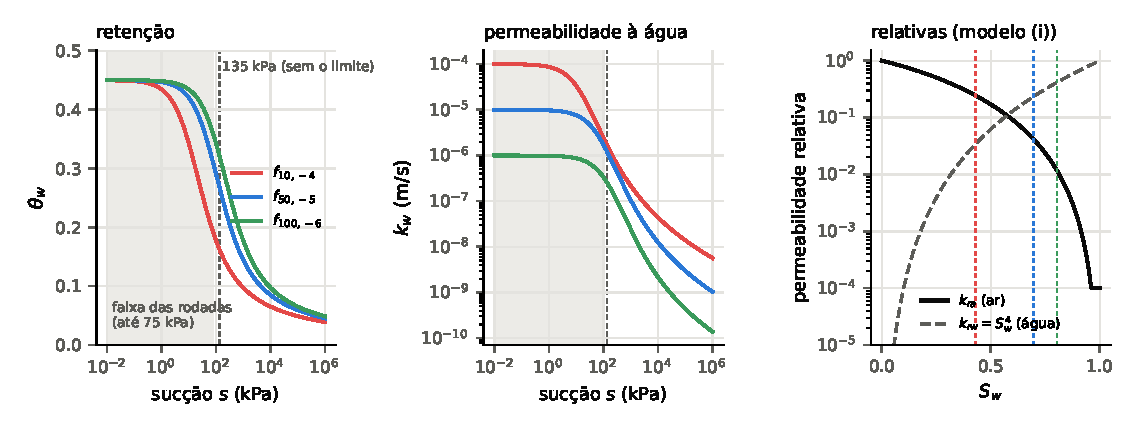
\includegraphics[width=\textwidth]{figs/solos.pdf}
\caption{Os três solos: a retenção $\theta_w(s)$ (a sucção inicial é limitada a 75~kPa), a permeabilidade à água
$k_w = k_s\Theta^4$, e as permeabilidades relativas contra $S_w$: ao ar (Brooks--Corey, $\lambda = 3$, piso
$10^{-4}$; só no modelo (i)) e à água ($S_w^4$). Cinza: a faixa de sucção das rodadas (até 75~kPa); tracejada: 135~kPa,
o máximo sem o limite. À direita, as verticais tracejadas são o menor $S_w$ das rodadas em cada solo.}\label{fig:solos}
\end{figure}

\paragraph{As rodadas.} Sete intensidades por solo (Tabela~2), múltiplos de $k_s$: $f_{10,-4}$ de $k_s/40 = 9$ a $2{,}5\,k_s
= 900$~mm/h; $f_{50,-5}$ de $k_s/10 = 3{,}6$ a $5\,k_s = 180$~mm/h; $f_{100,-6}$ de $k_s/4 = 0{,}9$ a $10\,k_s = 36$~mm/h.
As Figs.~6 e 7 têm mais 7 pontos ($f_{10,-4}$ a 0,9, 1,8 e 3,6; $f_{50,-5}$ a 0,9, 1,8 e 45; $f_{100,-6}$ a 0,36~mm/h),
também calculados aqui. A chuva dura 24~h e o FS vai até 48~h. Os marcadores da Fig.~5 estão em 0, 1, 2, 3, 6, 12, 24,
28, 32, 40 e 48~h: o FS mínimo do artigo é o menor desses instantes. Os valores do artigo foram lidos das figuras
(\texttt{data/}; erro de leitura de $\approx 0{,}02$, até $\approx 0{,}04$ entre 1 e 3~h, onde os marcadores se
sobrepõem).

\section{O modelo no NeoPZ}\label{sec:metodo}
\subsection{As leis de fluxo e os balanços de massa}\label{sec:fluxo}
As duas fases fluidas seguem a lei de Darcy generalizada, com a mesma permeabilidade intrínseca
$\kappa = k_s\mu_w/\gamma_w$ e as permeabilidades relativas da Seção~1 ($y$ para cima, $\mathbf g = -g\,\mathbf e_y$):
\begin{align}
\text{água:}\quad \mathbf q_w &= -\frac{\kappa\,k_{rw}}{\mu_w}\left(\nabla p_w - \rho_w\mathbf g\right)
  = -\frac{k_s\,k_{rw}(S_w)}{\gamma_w}\left(\nabla p_w + \gamma_w\,\mathbf e_y\right),\\
\text{ar:}\quad \mathbf q_a &= -\frac{\kappa\,k_{ra}}{\mu_a}\left(\nabla p_a - \rho_a\mathbf g\right)
  = -\frac{\mu_w}{\mu_a}\,\frac{k_s\,k_{ra}(S_w)}{\gamma_w}\left(\nabla p_a + \gamma_a\,\mathbf e_y\right),
\end{align}
com $\mathbf q_w$ e $\mathbf q_a$ relativos ao esqueleto, $\mu_w/\mu_a = 55{,}6$ e $\gamma_a = 0{,}0118$~kN/m$^3$. A
água em termos de carga é a forma usual: $\mathbf q_w = -k_w\nabla h$, com $h = y + p_w/\gamma_w$ e $k_w = k_s
k_{rw}$. A água é pouco compressível ($K_w = 2{,}2$~GPa) e o ar é gás ideal isotérmico ($\rho_a \propto p_a + p_{atm}$).
Para cada fluido $\pi\in\{w,a\}$, a massa por unidade de volume é $nS_\pi\rho_\pi$, e o seu balanço, em relação ao
esqueleto, é
\begin{equation}
\frac{1}{\rho_\pi}\frac{\mathrm d(nS_\pi\rho_\pi)}{\mathrm dt}+nS_\pi\,\dot\varepsilon_v
+\frac{1}{\rho_\pi}\nabla\!\cdot(\rho_\pi\mathbf q_\pi)=s_\pi,
\qquad
\mathbf q_\pi=-\lambda_\pi\big(\nabla p_\pi-\rho_\pi\mathbf g\big),\qquad \lambda_\pi = \frac{\kappa\,k_{r\pi}}{\mu_\pi},
\label{eq:massa-fase}
\end{equation}
com $s_\pi = 0$ aqui (sem fontes). Para chegar à forma que o código resolve:
\begin{itemize}
  \item \textbf{porosidade:} com grãos incompressíveis ($\alpha = 1$), $\dot n = (1-n)\,\dot\varepsilon_v$; então
    $S_\pi\dot n + nS_\pi\dot\varepsilon_v = S_\pi\dot\varepsilon_v$. Nos outros coeficientes $n = n_0 = 0{,}45$;
  \item \textbf{fluidos:} a água com $\dot\rho_w/\rho_w = \dot p_w/K_w$ ($K_w = 2{,}2$~GPa); o ar ideal isotérmico com
    $\dot\rho_a/\rho_a = \dot p_a/(p_a + p_{atm})$;
  \item \textbf{transporte:} $\rho_\pi^{-1}\nabla\!\cdot(\rho_\pi\mathbf q_\pi) = \nabla\!\cdot\mathbf q_\pi +
    c_\pi\,\mathbf q_\pi\cdot\nabla p_\pi$, com $c_w = 1/K_w$ (desprezado no código) e $c_a = 1/(p_a + p_{atm})$
    (mantido).
\end{itemize}
Assim:
\begin{align}
\text{água:}\quad & S_w\,\dot\varepsilon_v + n\,\dot S_w + \frac{n S_w}{K_w}\,\dot p_w + \nabla\!\cdot\mathbf q_w = 0,\\
\text{ar:}\quad & S_a\,\dot\varepsilon_v + n\,\dot S_a + \frac{n S_a}{p_a + p_{atm}}\,\dot p_a + \nabla\!\cdot\mathbf q_a
  + \frac{\mathbf q_a\cdot\nabla p_a}{p_a + p_{atm}} = 0,
\end{align}
com $S_a = 1 - S_w$ e $\dot S_w = -\Gamma\,(\dot p_a - \dot p_w)$, $\Gamma = -dS_w/ds$ a capacidade de retenção; o
equilíbrio mecânico está na Seção~\ref{sec:equil}. Os modelos usam essas equações assim:
\begin{itemize}
  \item \textbf{(iii)}: só o balanço da água, sem $\dot\varepsilon_v$ (esqueleto rígido) e com $p_a = 0$. É a equação de
    Richards do SEEP/W: $n\Gamma\,\dot p_w + (nS_w/K_w)\,\dot p_w + \nabla\!\cdot\mathbf q_w = 0$.
  \item \textbf{(ii)}: o balanço da água com $\dot\varepsilon_v$ e o equilíbrio (esqueleto elástico); $p_a = 0$.
  \item \textbf{(i)}: as três equações. No ar, $p_a = 0$ só na superfície; nas outras bordas o fluxo de ar é nulo.
\end{itemize}

\subsection{O equilíbrio mecânico}\label{sec:equil}
O esqueleto obedece ao equilíbrio quase estático, em deformação plana e pequenas deformações:
\begin{equation}
\nabla\!\cdot\boldsymbol\sigma + \rho_b\,\mathbf g = \mathbf 0,\qquad
\boldsymbol\varepsilon = \tfrac12\left[\nabla\mathbf u + (\nabla\mathbf u)^{\mathsf T}\right],\qquad
\varepsilon_v = \nabla\!\cdot\mathbf u,
\end{equation}
com o peso específico $\rho_b g = \gamma = 20$~kN/m$^3$ constante (acima e abaixo do nível, como no artigo). A tensão
total se divide pela tensão efetiva de Bishop (tração positiva, pressões positivas em compressão):
\begin{equation}
\boldsymbol\sigma = \boldsymbol\sigma' - \alpha\,p_B\,\mathbf I,\qquad
p_B = p_a - \chi\,(p_a - p_w) = p_a - \chi\,s,\qquad \alpha = 1.
\end{equation}
Aqui $\chi = \tan\phi^b/\tan\phi' = 1$, a escolha que reproduz a resistência de Fredlund do artigo (Eq.~5):
$p_B = p_w$, e a tensão efetiva é $\boldsymbol\sigma' = \boldsymbol\sigma + p_w\mathbf I$. O critério de Mohr--Coulomb em
$\boldsymbol\sigma'$ dá, num plano com tensão normal $\sigma_n$ (compressão positiva),
\begin{equation}
\tau_f = c' + (\sigma_n - p_w)\tan\phi' = c' + (\sigma_n - u_a)\tan\phi' + (u_a - u_w)\tan\phi^b,
\qquad \phi^b = \phi',
\end{equation}
que é a Eq.~5 do artigo. Com $\chi = 1$, $p_a$ sai da resistência: o ar só age através de $p_w$.
\begin{itemize}
  \item \textbf{Constitutivo:} $\boldsymbol\sigma'$ sai do Mohr--Coulomb associado ($c' = 10$~kPa, $\phi' = \psi =
    26°$) com a parte elástica isotrópica ($E = 20$~MPa, $\nu = 0{,}3$), retorno analítico e tangente consistente.
  \item \textbf{Contornos:} base presa ($u_x = u_y = 0$), laterais com $u_x = 0$, superfície livre.
  \item \textbf{No transiente:} o (iii) não resolve o equilíbrio (esqueleto rígido). No (ii) e no (i) ele é resolvido
    junto com os balanços de massa, com $c' = 10^9$ (resposta elástica) e a partir do estado geostático: o peso com as
    pressões iniciais, depois $\mathbf u = \mathbf 0$ com a tensão mantida. O termo $S_\pi\,\dot\varepsilon_v$ dos
    balanços de massa (Seção~\ref{sec:fluxo}) é o acoplamento de volta.
  \item \textbf{No fator de segurança:} as pressões de um instante ficam congeladas e só o equilíbrio é resolvido, com
    $c'/F$ e $\tan\phi'/F$ (Seção~\ref{sec:metodo}, SRM).
\end{itemize}

\subsection{O transiente}
\begin{itemize}
  \item \textbf{Material:} \texttt{TPZMatUnsaturatedUPwPa} (formulação $\mathbf u$--$p_w$--$p_a$), deformação plana,
    $\mathbf u$ quadrático e $p_w$, $p_a$ lineares. No modelo (iii) o acoplamento hidromecânico e a fase de ar estão
    desligados nas equações de massa (esqueleto rígido, $p_a = 0$): só a equação da água evolui (Richards), com o
    armazenamento concentrado nos vértices e $K_w = 2{,}2$~GPa.
  \item \textbf{Tempo:} Euler implícito com passo de 0,1~h (metades só se o Newton não converge), Newton com o
    jacobiano consistente, solver direto (LU esparsa).
  \item \textbf{Contornos:} os do artigo (carga nas laterais abaixo do nível inicial, fluxo nulo no resto). Na
    superfície, o fluxo $I_r$ por metro inclinado (o \emph{unit flux} do SEEP/W) com a condição unilateral $p_w \le 0$:
    o nó em que $p_w$ chegaria a 0 passa à face de percolação ($p_w = 0$) e volta ao fluxo quando a vazão pedida fica
    abaixo de $I_r$. O excesso escoa, como o artigo descreve.
  \item \textbf{Malha} (Fig.~\ref{fig:malhas}): camadas que seguem o terreno, colunas a cada 1~m, a primeira camada com
    0,3\,\% da altura da coluna (6 a 9~cm) crescendo 15\,\% até 2,5\,\% (0,5 a 0,75~m); 6860 triângulos, 35\,018
    equações.
\end{itemize}

\subsection{O fator de segurança: SRM}
\begin{itemize}
  \item \textbf{Definição:} o FS é o fator $F$ que leva o talude ao colapso quando a resistência é reduzida para
    $c'/F$ e $\tan\phi'/F$ (redução de resistência). Com $\chi = \tan\phi^b/\tan\phi' = 1$, a parcela da sucção,
    $\chi\,s\tan\phi'$, cai junto: é o $\tan\phi^b/F$ do Bishop, o mesmo fator do equilíbrio limite do artigo. A
    diferença é a superfície: livre no SRM, circular no Bishop simplificado.
  \item \textbf{Pressões congeladas:} em cada instante, $p_w$ do transiente é interpolada linearmente da malha do
    transiente para a do fator e fica fixa ($p_a = 0$); o fator resolve só o equilíbrio.
  \item \textbf{Material do fator:} Mohr--Coulomb associado ($\psi = \phi'$), retorno analítico e tangente consistente
    (\texttt{TPZPlasticStepVoigt<TPZYCMohrCoulombPV2>}), $E = 20$~MPa, $\nu = 0{,}3$ (não mudam o FS); $\mathbf u$
    quadrático. Cada análise parte do estado sem tensões.
  \item \textbf{Caminho:} (1) o peso é aplicado de 0 a 1 com $F = F_0 = 0{,}8$ (se o talude não fica em pé, $F_0/2$);
    (2) $F$ cresce por \emph{arc-length} cilíndrico, com a carga tangente $-\partial R/\partial F$ por diferença finita,
    até um patamar. O FS é o maior $F$ do caminho.
  \item \textbf{Refinamento adaptativo, refeito do zero em cada instante:} a malha inicial (catetos de 5~m) e 4
    níveis; em cada nível, os triângulos com $\sqrt{J_2(\boldsymbol\varepsilon^p)} \ge 0{,}1$ do maior (a banda de
    ruptura) são divididos e o SRM é refeito. O FS é o do último nível (Tabela~\ref{tab:niveis}).
  \item \textbf{Instantes:} de hora em hora, de 0 a 48~h (49 análises por rodada).
\end{itemize}

\begin{figure}[H]\centering
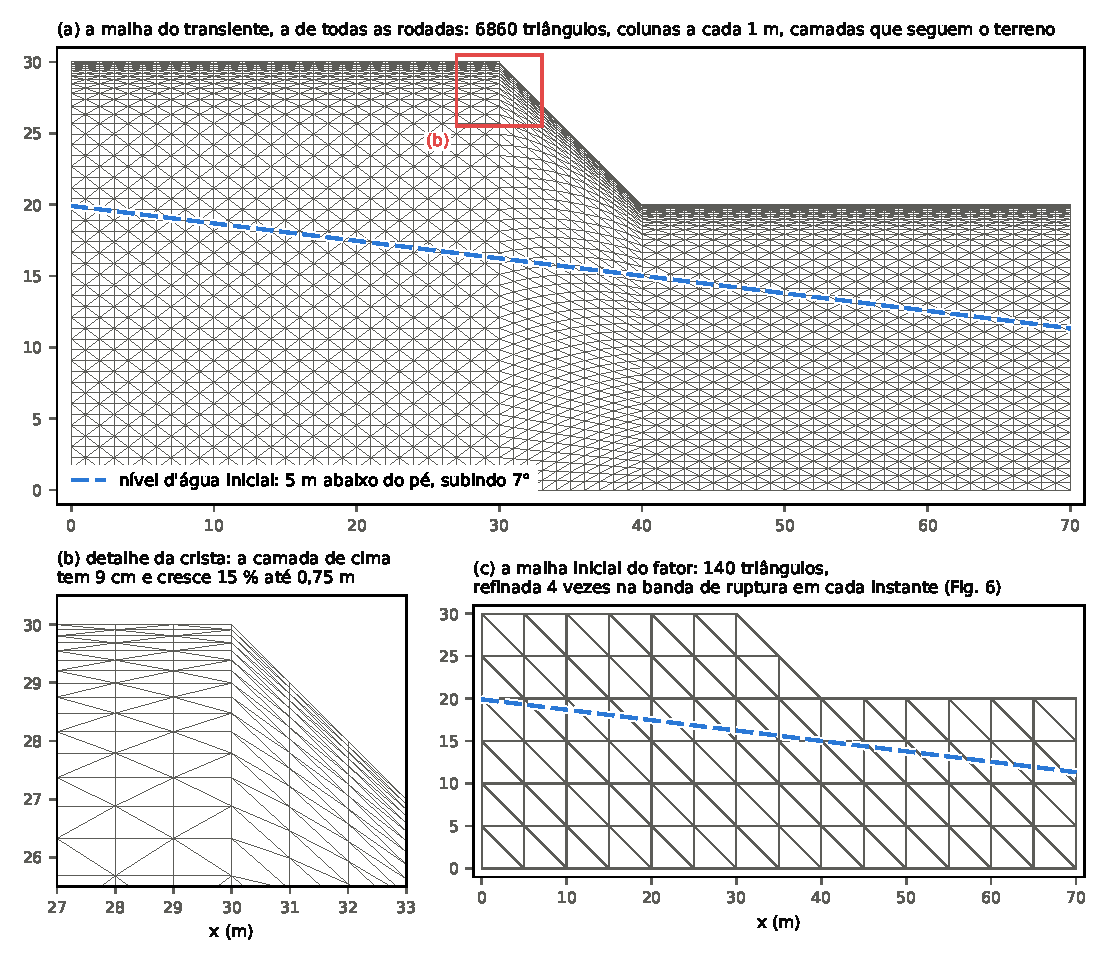
\includegraphics[width=0.92\textwidth]{figs/malhas.pdf}
\caption{As malhas. (a) A malha do transiente, a mesma em todas as rodadas (a conferência de malha da
Tabela~\ref{tab:malha} usa outra, com as colunas e as camadas pela metade: 25\,378 triângulos). (b) O detalhe da
crista: as camadas finas junto à superfície acompanham a frente de umedecimento. (c) A malha inicial do fator; em cada
instante ela é refinada 4 vezes na banda de ruptura (Fig.~\ref{fig:malhasF}). Tracejado: o nível d'água
inicial.}\label{fig:malhas}
\end{figure}

\paragraph{Conferência de malha.} Nos três casos extremos ($f_{10,-4}$ a 900, $f_{50,-5}$ e $f_{100,-6}$ a 36~mm/h), a
mesma rodada com a malha do transiente e o passo de tempo pela metade (colunas a cada 0,5~m, camadas de 0,15 a
1,25\,\%, $\Delta t = 0{,}05$~h; 25\,378 triângulos), nos instantes do artigo:

\begin{table}[H]\centering\scriptsize\setlength{\tabcolsep}{3pt}
\caption{O FS nos instantes do artigo com a malha base e com a malha e o passo pela metade (fina).}\label{tab:malha}
\resizebox{\textwidth}{!}{\begin{tabular}{l|ccccccccccc|c}
\toprule
caso & 0 h & 1 h & 2 h & 3 h & 6 h & 12 h & 24 h & 28 h & 32 h & 40 h & 48 h & máx. $|\Delta|$\\
\midrule
$f_{10,-4}$, 900 mm/h: base & 2{,}098 & 1{,}366 & 1{,}177 & 1{,}113 & 0{,}933 & 0{,}826 & 0{,}826 & 1{,}063 & 1{,}208 & 1{,}429 & 1{,}593 & \\
\phantom{$f_{10,-4}$, 900 mm/h:} fina & 2{,}099 & 1{,}357 & 1{,}174 & 1{,}113 & 0{,}926 & 0{,}826 & 0{,}826 & 1{,}063 & 1{,}206 & 1{,}428 & 1{,}593 & 0{,}008\\
$f_{50,-5}$, 36 mm/h: base & 2{,}098 & 2{,}037 & 1{,}981 & 1{,}924 & 1{,}722 & 1{,}398 & 1{,}030 & 1{,}087 & 1{,}128 & 1{,}202 & 1{,}264 & \\
\phantom{$f_{50,-5}$, 36 mm/h:} fina & 2{,}099 & 2{,}036 & 1{,}982 & 1{,}924 & 1{,}721 & 1{,}397 & 1{,}029 & 1{,}086 & 1{,}127 & 1{,}198 & 1{,}261 & 0{,}004\\
$f_{100,-6}$, 36 mm/h: base & 2{,}098 & 2{,}010 & 1{,}977 & 1{,}949 & 1{,}878 & 1{,}687 & 1{,}444 & 1{,}460 & 1{,}482 & 1{,}521 & 1{,}548 & \\
\phantom{$f_{100,-6}$, 36 mm/h:} fina & 2{,}099 & 2{,}011 & 1{,}977 & 1{,}949 & 1{,}879 & 1{,}686 & 1{,}442 & 1{,}459 & 1{,}482 & 1{,}521 & 1{,}548 & 0{,}001\\
\bottomrule
\end{tabular}
}
\end{table}

A malha e o passo pela metade mudam o FS em no máximo 0,008 (no $f_{10,-4}$ a 900~mm/h, em 1 e 6~h, quando a frente de
umedecimento ainda está nos primeiros metros); nos outros dois casos, em 0,004 e 0,001. O erro do transiente fica bem
abaixo do erro de leitura das figuras do artigo ($\approx 0{,}02$), e a malha base serve para as 28 rodadas e para o
modelo (i). (A malha fina tem 125\,978 equações e 960 passos: 55 a 65~min por rodada no PC, com 4 threads.)

\section{O FS ao longo do tempo (Fig.~5)}
\begin{figure}[H]\centering
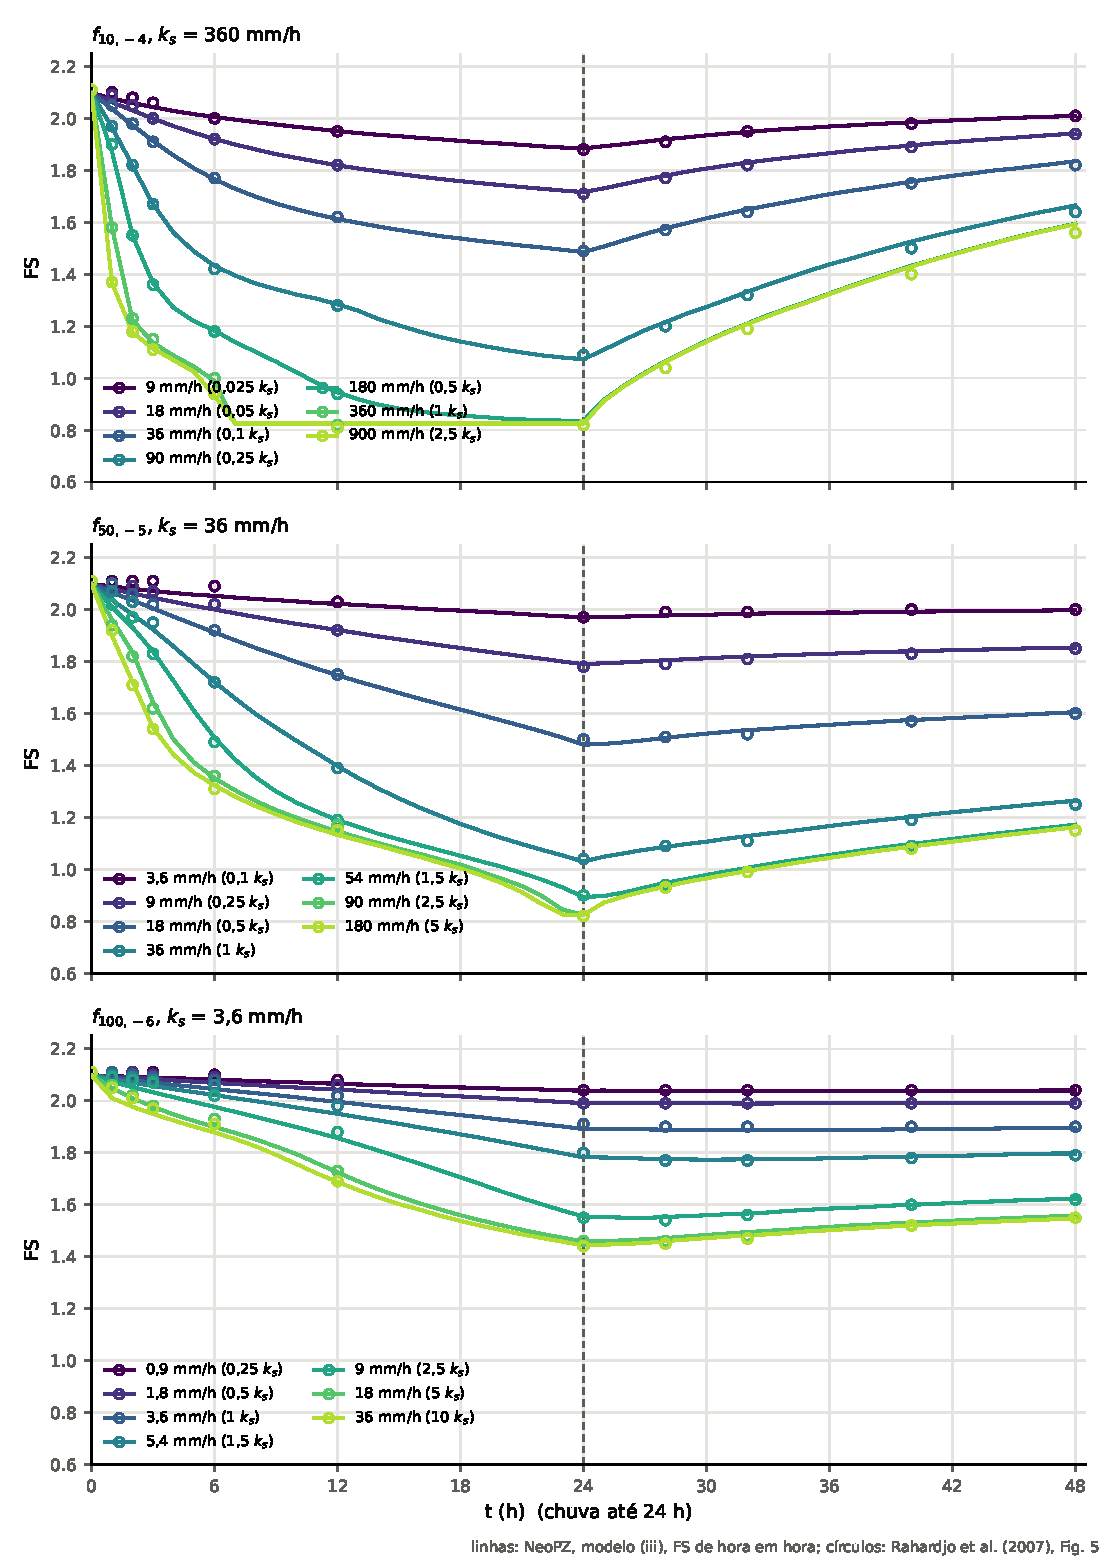
\includegraphics[width=0.9\textwidth]{figs/fs_tempo.pdf}
\caption{O FS contra o tempo nos três solos: o NeoPZ (modelo (iii), linhas, FS de hora em hora) e a Fig.~5 do artigo
(círculos). Chuva até 24~h (tracejado).}\label{fig:fs}
\end{figure}

As curvas do NeoPZ passam pelos marcadores do artigo nos três solos: dos \cincoN{} pontos da Fig.~5, \cincoFrac\,\%
ficam a até 0,03 e todos a até \cincoMax{} (desvio quadrático médio de \cincoRms). O que sobra tem padrão:
\begin{itemize}
  \item \textbf{Em 0~h} o nosso FS é 2,098 e o do artigo $\approx 2{,}11$, nos três solos (o estado inicial é o mesmo:
    a sucção limitada a 75~kPa não depende do solo). É a diferença entre os métodos: o SRM, com a superfície de
    ruptura livre, contra o círculo do Bishop simplificado.
  \item \textbf{Entre 1 e 6~h}, no $f_{50,-5}$ e no $f_{100,-6}$, os nossos pontos ficam até 0,05 abaixo. É onde os
    marcadores do artigo se sobrepõem e a leitura erra até 0,04.
  \item \textbf{No patamar saturado} ($f_{10,-4}$ de 180 a 900~mm/h e $f_{50,-5}$ a 90 e 180~mm/h, com o nível d'água
    na crista) o nosso FS é 0,826 e o do artigo 0,81. O FS do SRM ainda cai $\approx 0{,}01$ do nível 3 para o 4 do
    refinamento (Tabela~\ref{tab:niveis}): o FS convergido deve ficar perto de 0,815.
  \item \textbf{Depois da chuva} a recuperação também bate. O $f_{10,-4}$ recupera depressa: FS $\approx 1{,}6$ em
    48~h em todas as intensidades que saturaram o talude. O $f_{50,-5}$ recupera devagar, e o $f_{100,-6}$ quase nada.
    No $f_{100,-6}$ até 9~mm/h o FS ainda cai depois que a chuva para (o mínimo fica entre 27 e 35~h), porque a
    água que entrou continua descendo.
\end{itemize}

\section{O FS mínimo e a Eq.~6 (Figs.~6 e 7)}
\begin{figure}[H]\centering
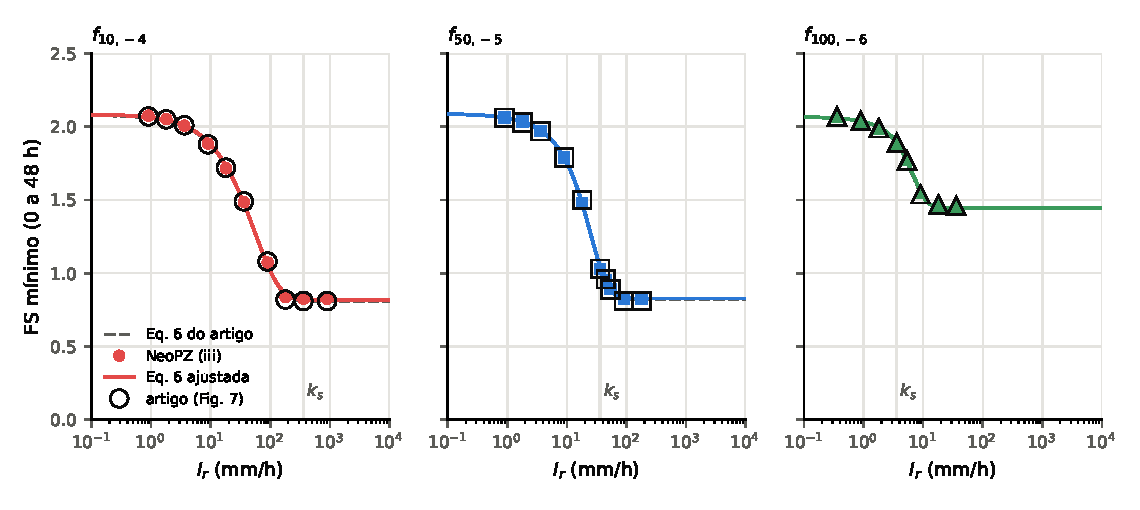
\includegraphics[width=\textwidth]{figs/fs_min.pdf}
\caption{O FS mínimo (0 a 48~h) contra a intensidade: o artigo (Fig.~7, vazios) com a sua Eq.~6 (tracejado), e o NeoPZ
(cheios) com a Eq.~6 ajustada aos nossos pontos.}\label{fig:fsmin}
\end{figure}

\begin{table}[H]\centering\scriptsize\setlength{\tabcolsep}{3pt}
\caption{O FS inicial e o FS mínimo, nosso e do artigo (Fig.~6), e a categoria do nível d'água no FS mínimo (Tabela~3
do artigo: I, o nível chega à crista; II, ao meio da face; III, ao pé; IV, não chega à superfície), nossa e do artigo
(Tabela~5). A nossa categoria é o ponto mais alto da superfície que o nível toca (Seção~\ref{sec:nivel}). ``Nos
instantes do artigo'': o nosso mínimo só entre 0, 1, 2, 3, 6, 12, 24, 28, 32, 40 e 48~h.}\label{tab:fsmin}
\resizebox{\textwidth}{!}{\begin{tabular}{lrr|ccc|ccc|cc}
\toprule
solo & $I_r$ & $I_r/k_s$ & \multicolumn{3}{c|}{FS inicial e FS mín.} & \multicolumn{3}{c|}{nosso: FS mín.} & \multicolumn{2}{c}{categoria}\\
 & (mm/h) & & nosso, 0 h & artigo & nosso & instante (h) & nos instantes & dif. & nossa & artigo\\
 & & & & (Fig. 6) & (0--48 h) & & do artigo & & & (Tab. 5)\\
\midrule
$f_{10,-4}$ & 0{,}9 & 0{,}0025 & 2{,}098 & 2{,}07 & 2{,}076 & 25 & 2{,}076 & $+$0{,}01 & IV & --\\
$f_{10,-4}$ & 1{,}8 & 0{,}005 & 2{,}098 & 2{,}05 & 2{,}052 & 24 & 2{,}052 & 0{,}00 & IV & --\\
$f_{10,-4}$ & 3{,}6 & 0{,}01 & 2{,}098 & 2{,}01 & 2{,}007 & 24 & 2{,}007 & 0{,}00 & IV & --\\
$f_{10,-4}$ & 9 & 0{,}025 & 2{,}098 & 1{,}88 & 1{,}884 & 24 & 1{,}884 & 0{,}00 & IV & IV\\
$f_{10,-4}$ & 18 & 0{,}05 & 2{,}098 & 1{,}72 & 1{,}716 & 24 & 1{,}716 & 0{,}00 & IV & IV\\
$f_{10,-4}$ & 36 & 0{,}1 & 2{,}098 & 1{,}49 & 1{,}486 & 24 & 1{,}486 & 0{,}00 & IV & IV\\
$f_{10,-4}$ & 90 & 0{,}25 & 2{,}098 & 1{,}08 & 1{,}073 & 24 & 1{,}073 & $-$0{,}01 & III & III\\
$f_{10,-4}$ & 180 & 0{,}5 & 2{,}098 & 0{,}82 & 0{,}836 & 24 & 0{,}836 & $+$0{,}02 & I & I\\
$f_{10,-4}$ & 360 & 1 & 2{,}098 & 0{,}81 & 0{,}826 & 8 & 0{,}826 & $+$0{,}02 & I & I\\
$f_{10,-4}$ & 900 & 2{,}5 & 2{,}098 & 0{,}81 & 0{,}826 & 7 & 0{,}826 & $+$0{,}02 & I & I\\
\midrule
$f_{50,-5}$ & 0{,}9 & 0{,}025 & 2{,}098 & 2{,}06 & 2{,}064 & 24 & 2{,}064 & 0{,}00 & IV & --\\
$f_{50,-5}$ & 1{,}8 & 0{,}05 & 2{,}098 & 2{,}03 & 2{,}034 & 24 & 2{,}034 & 0{,}00 & IV & --\\
$f_{50,-5}$ & 3{,}6 & 0{,}1 & 2{,}098 & 1{,}97 & 1{,}971 & 24 & 1{,}971 & 0{,}00 & IV & IV\\
$f_{50,-5}$ & 9 & 0{,}25 & 2{,}098 & 1{,}79 & 1{,}790 & 24 & 1{,}790 & 0{,}00 & IV & IV\\
$f_{50,-5}$ & 18 & 0{,}5 & 2{,}098 & 1{,}50 & 1{,}480 & 24 & 1{,}480 & $-$0{,}02 & IV & IV\\
$f_{50,-5}$ & 36 & 1 & 2{,}098 & 1{,}03 & 1{,}030 & 24 & 1{,}030 & 0{,}00 & II & II\\
$f_{50,-5}$ & 45 & 1{,}25 & 2{,}098 & 0{,}96 & 0{,}951 & 24 & 0{,}951 & $-$0{,}01 & II & --\\
$f_{50,-5}$ & 54 & 1{,}5 & 2{,}098 & 0{,}89 & 0{,}894 & 24 & 0{,}894 & 0{,}00 & I & I\\
$f_{50,-5}$ & 90 & 2{,}5 & 2{,}098 & 0{,}81 & 0{,}826 & 24 & 0{,}826 & $+$0{,}02 & I & I\\
$f_{50,-5}$ & 180 & 5 & 2{,}098 & 0{,}81 & 0{,}826 & 24 & 0{,}826 & $+$0{,}02 & I & I\\
\midrule
$f_{100,-6}$ & 0{,}36 & 0{,}1 & 2{,}098 & 2{,}07 & 2{,}065 & 33 & 2{,}067 & 0{,}00 & IV & --\\
$f_{100,-6}$ & 0{,}9 & 0{,}25 & 2{,}098 & 2{,}04 & 2{,}036 & 31 & 2{,}037 & 0{,}00 & IV & IV\\
$f_{100,-6}$ & 1{,}8 & 0{,}5 & 2{,}098 & 1{,}99 & 1{,}989 & 32 & 1{,}989 & 0{,}00 & IV & IV\\
$f_{100,-6}$ & 3{,}6 & 1 & 2{,}098 & 1{,}89 & 1{,}886 & 35 & 1{,}888 & 0{,}00 & IV & IV\\
$f_{100,-6}$ & 5{,}4 & 1{,}5 & 2{,}098 & 1{,}77 & 1{,}773 & 30 & 1{,}774 & 0{,}00 & IV & IV\\
$f_{100,-6}$ & 9 & 2{,}5 & 2{,}098 & 1{,}54 & 1{,}549 & 27 & 1{,}552 & $+$0{,}01 & IV & IV\\
$f_{100,-6}$ & 18 & 5 & 2{,}098 & 1{,}47 & 1{,}458 & 24 & 1{,}458 & $-$0{,}01 & IV & IV\\
$f_{100,-6}$ & 36 & 10 & 2{,}098 & 1{,}46 & 1{,}444 & 24 & 1{,}444 & $-$0{,}02 & IV & IV\\
\bottomrule
\end{tabular}
}
\end{table}

\begin{table}[H]\centering\small
\caption{A Eq.~6, $F_{s(min)} = A + B/\{1 + \exp[-(I_r - C)/D]\}$ ($I_r$ em mm/h): os parâmetros do artigo (Fig.~7) e os
ajustados aos nossos pontos. $I_{r(ini)}$ e $I_{r(thr)}$: as intensidades em que a tangente ao trecho inclinado da curva
(no gráfico semilog) cruza o patamar de cima e o de baixo; entre parênteses, a mesma construção aplicada à Eq.~6 do
artigo (ele traçou as tangentes à mão). $^\dagger$: $C$ fixo no valor do artigo (com $C < 0$ só $B\,e^{C/|D|}$ é
identificável).}\label{tab:eq6}
\begin{tabular}{ll|cccc|c|cc}
\toprule
solo & & $A$ & $B$ & $C$ & $D$ & $r^2$ & $I_{r(ini)}$ (mm/h) & $I_{r(thr)}$ (mm/h)\\
\midrule
$f_{10,-4}$ & artigo & 0{,}81 & 13{,}54 & -118 & -52 & 0{,}999 & 11 (10{,}37) & 140 (146{,}44)\\
 & NeoPZ (10 pontos) & 0{,}82 & 13{,}92 & -118$^\dagger$ & -51{,}25 & 0{,}999 & 10{,}19 & 144{,}17\\
\midrule
$f_{50,-5}$ & artigo & 0{,}82 & 1{,}83 & 10{,}7 & -13{,}13 & 0{,}997 & 8{,}5 (7{,}31) & 51 (50{,}42)\\
 & NeoPZ (10 pontos) & 0{,}83 & 1{,}82 & 10{,}48 & -12{,}77 & 1{,}000 & 7{,}13 & 49{,}07\\
\midrule
$f_{100,-6}$ & artigo & 1{,}45 & 0{,}70 & 4{,}75 & -2{,}35 & 0{,}998 & 2{,}8 (2{,}57) & 11 (11{,}08)\\
 & NeoPZ (8 pontos) & 1{,}45 & 0{,}71 & 4{,}87 & -2{,}43 & 0{,}999 & 2{,}63 & 11{,}42\\
\bottomrule
\end{tabular}

\end{table}

Os \nCasos{} FS mínimos ficam a até \difMax{} dos do artigo (diferença média \difMedia). A sigmoide da Fig.~7 sai
inteira, com os dois patamares e o trecho inclinado no mesmo lugar. A Eq.~6 ajustada aos nossos pontos
(Tabela~\ref{tab:eq6}):
\begin{itemize}
  \item \textbf{$f_{50,-5}$ e $f_{100,-6}$:} os quatro parâmetros livres ficam a até 3,5\,\% dos do artigo.
  \item \textbf{$f_{10,-4}$:} o $C$ do artigo é negativo ($-118$~mm/h). Com $C < 0$, para $I_r \ge 0$, a Eq.~6 é
    praticamente $A + B\,e^{C/|D|}\,e^{-I_r/|D|}$. Só o produto $B\,e^{C/|D|}$ conta, e o ajuste livre vai a
    $B \approx 2{,}6\times10^4$ e $C \approx -540$ com a mesma curva; o mesmo acontece ajustando os pontos lidos do
    próprio artigo. Com $C$ fixo em $-118$: $A = 0{,}82$, $B = 13{,}9$ e $D = -51{,}2$ (artigo: 0,81, 13,54 e $-52$).
  \item \textbf{O patamar de baixo}, $A$, é o FS do talude saturado até a crista: 0,82 a 0,83, contra 0,81 e 0,82 no
    artigo, igual nos dois solos que saturam. No $f_{100,-6}$ o nível não chega à superfície e o patamar de baixo é
    outro: 1,45, como no artigo. Ali a chuva só tira a sucção das camadas de cima (Seção~\ref{sec:campos}).
  \item \textbf{$I_{r(ini)}$ e $I_{r(thr)}$:} 10,2 e 144~mm/h (artigo: 11 e 140), 7,1 e 49 (8,5 e 51) e 2,6 e 11,4
    (2,8 e 11). Comparando com a mesma construção aplicada à Eq.~6 do artigo (entre parênteses na tabela), as
    diferenças ficam abaixo de 0,2~mm/h em $I_{r(ini)}$ e de 3\,\% em $I_{r(thr)}$. O resto é o traçado à mão do
    artigo.
  \item \textbf{Em múltiplos de $k_s$}, $I_{r(thr)}$ é $0{,}4\,k_s$ no $f_{10,-4}$, $1{,}4\,k_s$ no $f_{50,-5}$ e
    $3{,}2\,k_s$ no $f_{100,-6}$. Em 24~h de chuva, o solo mais permeável chega ao patamar de baixo com uma fração de
    $k_s$; o menos permeável precisa de várias vezes $k_s$, e mesmo assim o patamar é só o da perda de sucção.
\end{itemize}

\section{O nível d'água no FS mínimo (Tabela~5)}\label{sec:nivel}
\begin{figure}[H]\centering
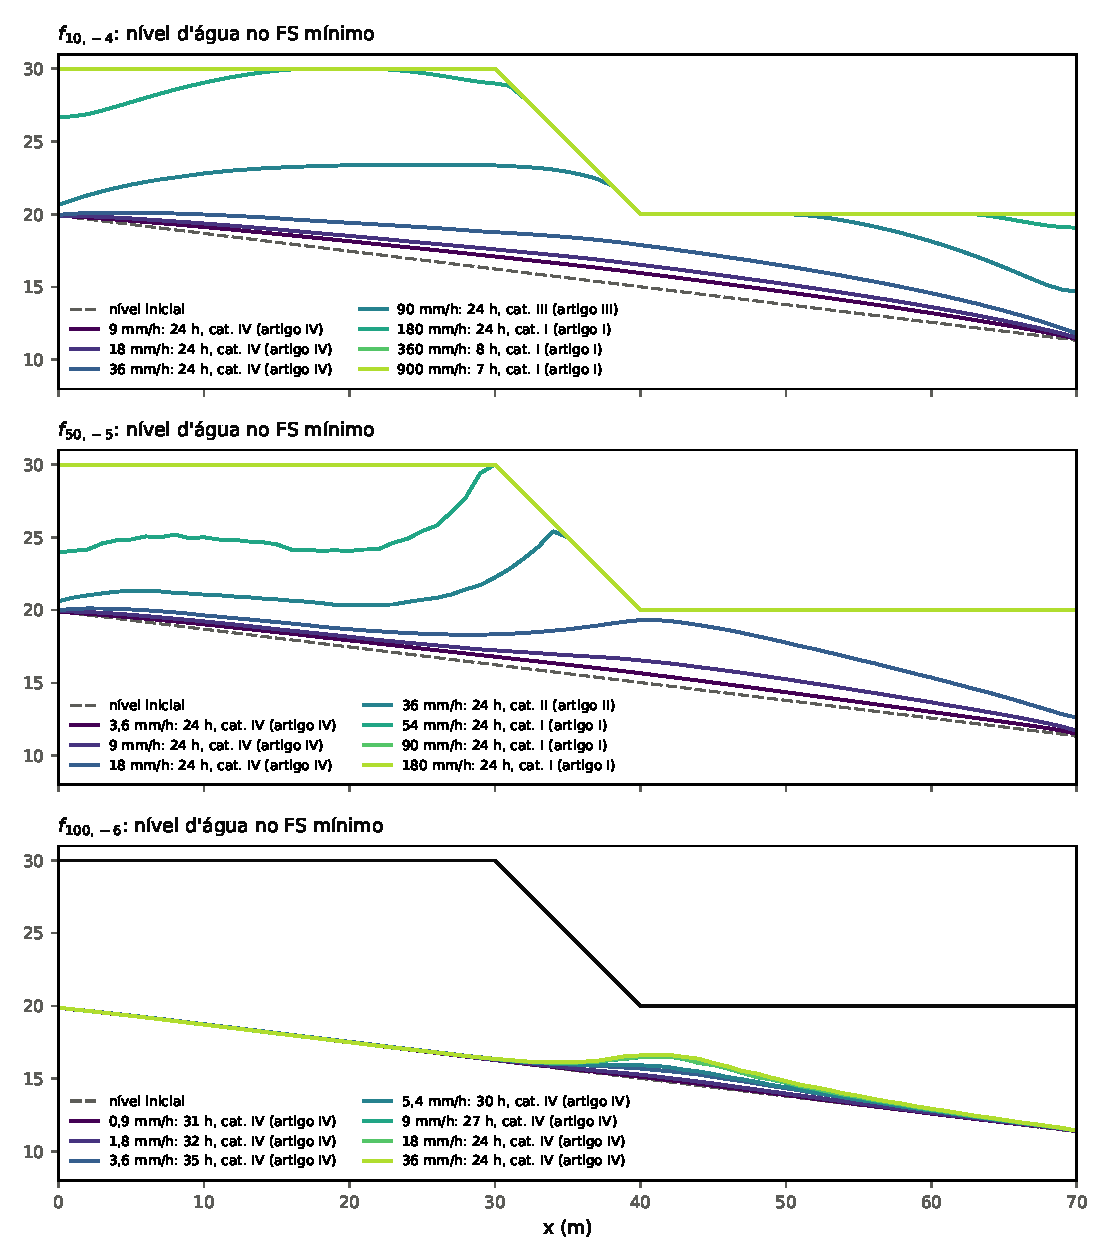
\includegraphics[width=0.92\textwidth]{figs/nivel.pdf}
\caption{O nível d'água (o topo da zona saturada que vem da base) no instante do FS mínimo, e a categoria da Tabela~3:
nossa e, entre parênteses, a da Tabela~5 do artigo.}\label{fig:nivel}
\end{figure}

As \catOk{} de \catTot{} categorias da Tabela~5 saem iguais (Tabela~\ref{tab:fsmin}). A regra: a categoria é o ponto
mais alto da superfície que o nível d'água toca (a menos de 5~cm) no instante do FS mínimo. A crista ($x \le 30$~m) dá
I, a metade de cima da face ($x \le 35$~m) dá II, o resto da face e o pé dão III, e não tocar dá IV. O programa
(\texttt{Categoria} em \texttt{main.cpp}) testa só três pontos ($x = 30$, 35 e 40~m) e dá II para o $f_{10,-4}$ a
180~mm/h. Ali o nível fica 1~m abaixo da quina da crista, porque a água drena para a face, mas já está na superfície
de $x = 16$ a 28~m (Fig.~\ref{fig:nivel}).

Os solos se separam pelo nível d'água em 24~h (Tabela~\ref{tab:diag}):
\begin{itemize}
  \item \textbf{$f_{10,-4}$:} até 36~mm/h ($k_s/10$) o nível sobe até 3~m e não chega à superfície; a 90~mm/h chega
    ao pé, e de 180~mm/h para cima, à crista.
  \item \textbf{$f_{50,-5}$:} até 18~mm/h ($k_s/2$) não chega (a 18~mm/h fica 0,7~m abaixo do pé); a 36 e 45~mm/h
    chega à metade de cima da face; de 54~mm/h para cima, à crista.
  \item \textbf{$f_{100,-6}$:} o nível mal sai do lugar (sobe no máximo 1,6~m, junto ao pé) e fica na categoria IV em
    todas as intensidades.
\end{itemize}

\paragraph{O refinamento do fator.} O FS em cada nível do refinamento adaptativo, no instante do FS mínimo das 21
rodadas da Fig.~5:

\begin{table}[H]\centering\small
\caption{O FS em cada nível do refinamento adaptativo do SRM, no instante do FS mínimo.}\label{tab:niveis}
\begin{tabular}{lr|ccccc|c}
\toprule
solo & $I_r$ & nível 0 & 1 & 2 & 3 & 4 & 4 $-$ 3\\
\midrule
$f_{10,-4}$ & 9 & 2{,}029 & 1{,}920 & 1{,}899 & 1{,}889 & 1{,}884 & -0{,}004\\
$f_{10,-4}$ & 18 & 1{,}879 & 1{,}765 & 1{,}734 & 1{,}722 & 1{,}716 & -0{,}006\\
$f_{10,-4}$ & 36 & 1{,}658 & 1{,}546 & 1{,}508 & 1{,}493 & 1{,}486 & -0{,}008\\
$f_{10,-4}$ & 90 & 1{,}251 & 1{,}135 & 1{,}093 & 1{,}078 & 1{,}073 & -0{,}005\\
$f_{10,-4}$ & 180 & 1{,}012 & 0{,}919 & 0{,}867 & 0{,}845 & 0{,}836 & -0{,}009\\
$f_{10,-4}$ & 360 & 0{,}998 & 0{,}908 & 0{,}859 & 0{,}835 & 0{,}826 & -0{,}010\\
$f_{10,-4}$ & 900 & 0{,}998 & 0{,}908 & 0{,}859 & 0{,}835 & 0{,}826 & -0{,}010\\
$f_{50,-5}$ & 3{,}6 & 2{,}108 & 2{,}003 & 1{,}983 & 1{,}973 & 1{,}971 & -0{,}002\\
$f_{50,-5}$ & 9 & 1{,}934 & 1{,}827 & 1{,}805 & 1{,}794 & 1{,}790 & -0{,}004\\
$f_{50,-5}$ & 18 & 1{,}620 & 1{,}521 & 1{,}492 & 1{,}483 & 1{,}480 & -0{,}003\\
$f_{50,-5}$ & 36 & 1{,}227 & 1{,}115 & 1{,}062 & 1{,}040 & 1{,}030 & -0{,}010\\
$f_{50,-5}$ & 54 & 1{,}071 & 0{,}982 & 0{,}927 & 0{,}904 & 0{,}894 & -0{,}011\\
$f_{50,-5}$ & 90 & 0{,}998 & 0{,}908 & 0{,}859 & 0{,}835 & 0{,}826 & -0{,}010\\
$f_{50,-5}$ & 180 & 0{,}998 & 0{,}908 & 0{,}859 & 0{,}835 & 0{,}826 & -0{,}010\\
$f_{100,-6}$ & 0{,}9 & 2{,}186 & 2{,}076 & 2{,}052 & 2{,}041 & 2{,}036 & -0{,}005\\
$f_{100,-6}$ & 1{,}8 & 2{,}144 & 2{,}029 & 2{,}004 & 1{,}994 & 1{,}989 & -0{,}005\\
$f_{100,-6}$ & 3{,}6 & 2{,}059 & 1{,}937 & 1{,}908 & 1{,}892 & 1{,}886 & -0{,}006\\
$f_{100,-6}$ & 5{,}4 & 1{,}966 & 1{,}841 & 1{,}796 & 1{,}780 & 1{,}773 & -0{,}007\\
$f_{100,-6}$ & 9 & 1{,}804 & 1{,}673 & 1{,}593 & 1{,}564 & 1{,}549 & -0{,}015\\
$f_{100,-6}$ & 18 & 1{,}618 & 1{,}545 & 1{,}493 & 1{,}470 & 1{,}458 & -0{,}012\\
$f_{100,-6}$ & 36 & 1{,}605 & 1{,}531 & 1{,}479 & 1{,}455 & 1{,}444 & -0{,}012\\
\bottomrule
\end{tabular}

\end{table}

Do nível 3 para o 4 o FS ainda cai de 0,002 a 0,015, e a queda diminui mais ou menos pela metade a cada nível. Por esse
critério o FS convergido fica cerca de 0,01 abaixo do último nível. É um viés pequeno e sempre para cima; para comparar
os modelos (iii) e (i) basta usar o mesmo refinamento nos dois.

\section{O transiente e a primeira passagem}\label{sec:trans}
\begin{table}[H]\centering\small
\caption{O transiente: o FS em 0, 24 e 48~h; a fração da chuva até 24~h que infiltrou (a chuva por metro inclinado,
74,1~m de superfície); a hora em que a superfície começa a alagar (face de percolação); o nível d'água em 24~h na
crista ($x = 30$~m, superfície em 30~m), no meio da face (25~m) e no pé (20~m).}\label{tab:diag}
\resizebox{\textwidth}{!}{\begin{tabular}{lr|ccc|cc|ccc}
\toprule
 & & \multicolumn{3}{c|}{FS} & \multicolumn{2}{c|}{chuva até 24 h} & \multicolumn{3}{c}{nível d'água em 24 h (m)}\\
solo & $I_r$ & 0 h & 24 h & 48 h & infiltrou & alaga em & crista & meio & pé\\
 & (mm/h) & & & & (\%) & (h) & (30) & (25) & (20)\\
\midrule
$f_{10,-4}$ & 0{,}9 & 2{,}098 & 2{,}076 & 2{,}081 & 100 & -- & 16{,}72 & 16{,}12 & 15{,}50\\
$f_{10,-4}$ & 1{,}8 & 2{,}098 & 2{,}052 & 2{,}072 & 100 & -- & 16{,}76 & 16{,}16 & 15{,}55\\
$f_{10,-4}$ & 3{,}6 & 2{,}098 & 2{,}007 & 2{,}056 & 100 & -- & 16{,}84 & 16{,}25 & 15{,}64\\
$f_{10,-4}$ & 9 & 2{,}098 & 1{,}884 & 2{,}010 & 100 & -- & 17{,}10 & 16{,}56 & 15{,}96\\
$f_{10,-4}$ & 18 & 2{,}098 & 1{,}716 & 1{,}942 & 100 & -- & 17{,}59 & 17{,}10 & 16{,}53\\
$f_{10,-4}$ & 36 & 2{,}098 & 1{,}486 & 1{,}835 & 100 & -- & 18{,}77 & 18{,}43 & 17{,}88\\
$f_{10,-4}$ & 90 & 2{,}098 & 1{,}073 & 1{,}665 & 94 & 14 & 23{,}36 & 22{,}92 & 20{,}00\\
$f_{10,-4}$ & 180 & 2{,}098 & 0{,}836 & 1{,}595 & 73 & 7 & 28{,}99 & 25{,}00 & 20{,}00\\
$f_{10,-4}$ & 360 & 2{,}098 & 0{,}826 & 1{,}593 & 42 & 2 & 30{,}00 & 25{,}00 & 20{,}00\\
$f_{10,-4}$ & 900 & 2{,}098 & 0{,}826 & 1{,}593 & 17 & 1 & 30{,}00 & 25{,}00 & 20{,}00\\
$f_{50,-5}$ & 0{,}9 & 2{,}098 & 2{,}064 & 2{,}069 & 100 & -- & 16{,}60 & 15{,}96 & 15{,}30\\
$f_{50,-5}$ & 1{,}8 & 2{,}098 & 2{,}034 & 2{,}047 & 100 & -- & 16{,}67 & 16{,}05 & 15{,}42\\
$f_{50,-5}$ & 3{,}6 & 2{,}098 & 1{,}971 & 1{,}997 & 100 & -- & 16{,}80 & 16{,}24 & 15{,}66\\
$f_{50,-5}$ & 9 & 2{,}098 & 1{,}790 & 1{,}853 & 100 & -- & 17{,}23 & 16{,}90 & 16{,}54\\
$f_{50,-5}$ & 18 & 2{,}098 & 1{,}480 & 1{,}605 & 100 & -- & 18{,}33 & 18{,}68 & 19{,}31\\
$f_{50,-5}$ & 36 & 2{,}098 & 1{,}030 & 1{,}264 & 87 & 12 & 22{,}24 & 25{,}00 & 20{,}00\\
$f_{50,-5}$ & 45 & 2{,}098 & 0{,}951 & 1{,}194 & 78 & 9 & 25{,}53 & 25{,}00 & 20{,}00\\
$f_{50,-5}$ & 54 & 2{,}098 & 0{,}894 & 1{,}172 & 68 & 6 & 30{,}00 & 25{,}00 & 20{,}00\\
$f_{50,-5}$ & 90 & 2{,}098 & 0{,}826 & 1{,}162 & 42 & 2 & 30{,}00 & 25{,}00 & 20{,}00\\
$f_{50,-5}$ & 180 & 2{,}098 & 0{,}826 & 1{,}162 & 21 & 1 & 30{,}00 & 25{,}00 & 20{,}00\\
$f_{100,-6}$ & 0{,}36 & 2{,}098 & 2{,}068 & 2{,}067 & 100 & -- & 16{,}25 & 15{,}64 & 15{,}04\\
$f_{100,-6}$ & 0{,}9 & 2{,}098 & 2{,}039 & 2{,}039 & 100 & -- & 16{,}25 & 15{,}65 & 15{,}07\\
$f_{100,-6}$ & 1{,}8 & 2{,}098 & 1{,}991 & 1{,}993 & 100 & -- & 16{,}26 & 15{,}67 & 15{,}14\\
$f_{100,-6}$ & 3{,}6 & 2{,}098 & 1{,}891 & 1{,}896 & 100 & -- & 16{,}27 & 15{,}72 & 15{,}30\\
$f_{100,-6}$ & 5{,}4 & 2{,}098 & 1{,}782 & 1{,}797 & 100 & -- & 16{,}28 & 15{,}79 & 15{,}49\\
$f_{100,-6}$ & 9 & 2{,}098 & 1{,}555 & 1{,}624 & 95 & 11 & 16{,}31 & 15{,}94 & 16{,}00\\
$f_{100,-6}$ & 18 & 2{,}098 & 1{,}458 & 1{,}558 & 56 & 3 & 16{,}35 & 16{,}09 & 16{,}50\\
$f_{100,-6}$ & 36 & 2{,}098 & 1{,}444 & 1{,}548 & 29 & 1 & 16{,}36 & 16{,}13 & 16{,}60\\
\bottomrule
\end{tabular}
}
\end{table}

\paragraph{Primeira passagem.} O instante $t_1$ em que o FS cruza 1 pela primeira vez (interpolado entre as horas
vizinhas) é a ruptura: o que vem depois no cálculo usa a geometria intacta e as pressões de um talude que já rompeu. Com
chuva constante, $t_1$ dá a ruptura para todas as durações: a rodada que rompe em $t_1$ rompe em qualquer chuva da
mesma intensidade com duração $D \ge t_1$.

\begin{table}[H]\centering\small
\caption{As rodadas que rompem: $t_1$ (o FS cruza 1 descendo), o instante em que volta acima de 1 e o tempo abaixo de
1.}\label{tab:cruza}
\begin{tabular}{lr|ccc}
\toprule
solo & $I_r$ (mm/h) & $t_1$ (h) & volta (h) & abaixo de 1 (h)\\
\midrule
$f_{10,-4}$ & 180 & 10{,}55 & 26{,}56 & 16{,}01\\
$f_{10,-4}$ & 360 & 5{,}80 & 26{,}62 & 20{,}81\\
$f_{10,-4}$ & 900 & 5{,}27 & 26{,}62 & 21{,}35\\
$f_{50,-5}$ & 45 & 21{,}94 & 29{,}26 & 7{,}32\\
$f_{50,-5}$ & 54 & 20{,}42 & 31{,}55 & 11{,}14\\
$f_{50,-5}$ & 90 & 18{,}68 & 32{,}45 & 13{,}77\\
$f_{50,-5}$ & 180 & 18{,}13 & 32{,}45 & 14{,}31\\
\bottomrule
\end{tabular}

\end{table}

\begin{itemize}
  \item \textbf{Infiltração:} a chuva entra inteira até 36~mm/h ($k_s/10$) no $f_{10,-4}$, até 18~mm/h ($k_s/2$) no
    $f_{50,-5}$ e até 5,4~mm/h ($1{,}5\,k_s$) no $f_{100,-6}$. Acima disso a superfície alaga e o excesso escoa. No
    $f_{10,-4}$ a 900~mm/h só 17\,\% entra, e a superfície alaga já na primeira hora.
  \item \textbf{Ruptura:} rompem (FS $< 1$) as três intensidades mais fortes do $f_{10,-4}$ (180, 360 e 900~mm/h,
    $t_1$ = 10,6, 5,8 e 5,3~h) e as quatro mais fortes do $f_{50,-5}$ (45 a 180~mm/h, $t_1$ = 21,9 a 18,1~h). O
    $f_{100,-6}$ não rompe. Acima de $I_{r(thr)}$ o $t_1$ quase não muda (de 5,8 para 5,3~h no $f_{10,-4}$, de 18,7
    para 18,1~h no $f_{50,-5}$), porque o que passa da capacidade de infiltração escoa.
  \item \textbf{Depois da chuva:} o FS volta acima de 1 em 2,6~h no $f_{10,-4}$ e em 5 a 8,5~h no $f_{50,-5}$.
  \item \textbf{Duração crítica:} nas rodadas que rompem, o FS começa a subir assim que a chuva para (o mínimo cai em
    24~h ou no patamar). Então $t_1$ é também, com boa aproximação, a menor duração de chuva que rompe o talude naquela
    intensidade: 22~h a 45~mm/h no $f_{50,-5}$, 10,6~h a 180~mm/h no $f_{10,-4}$. Cada rodada que rompe dá um ponto da
    curva intensidade--duração crítica.
\end{itemize}

\section{Campos de pressão e malhas do fator}\label{sec:campos}
Seis rodadas no PC (duas intensidades por solo, com o FS em 0, 6, 12, 24 e 48~h) gravam o campo de $p_w$ e a malha
final do fator em cada instante.

\ifnum\nCampos>0
\begin{figure}[H]\centering
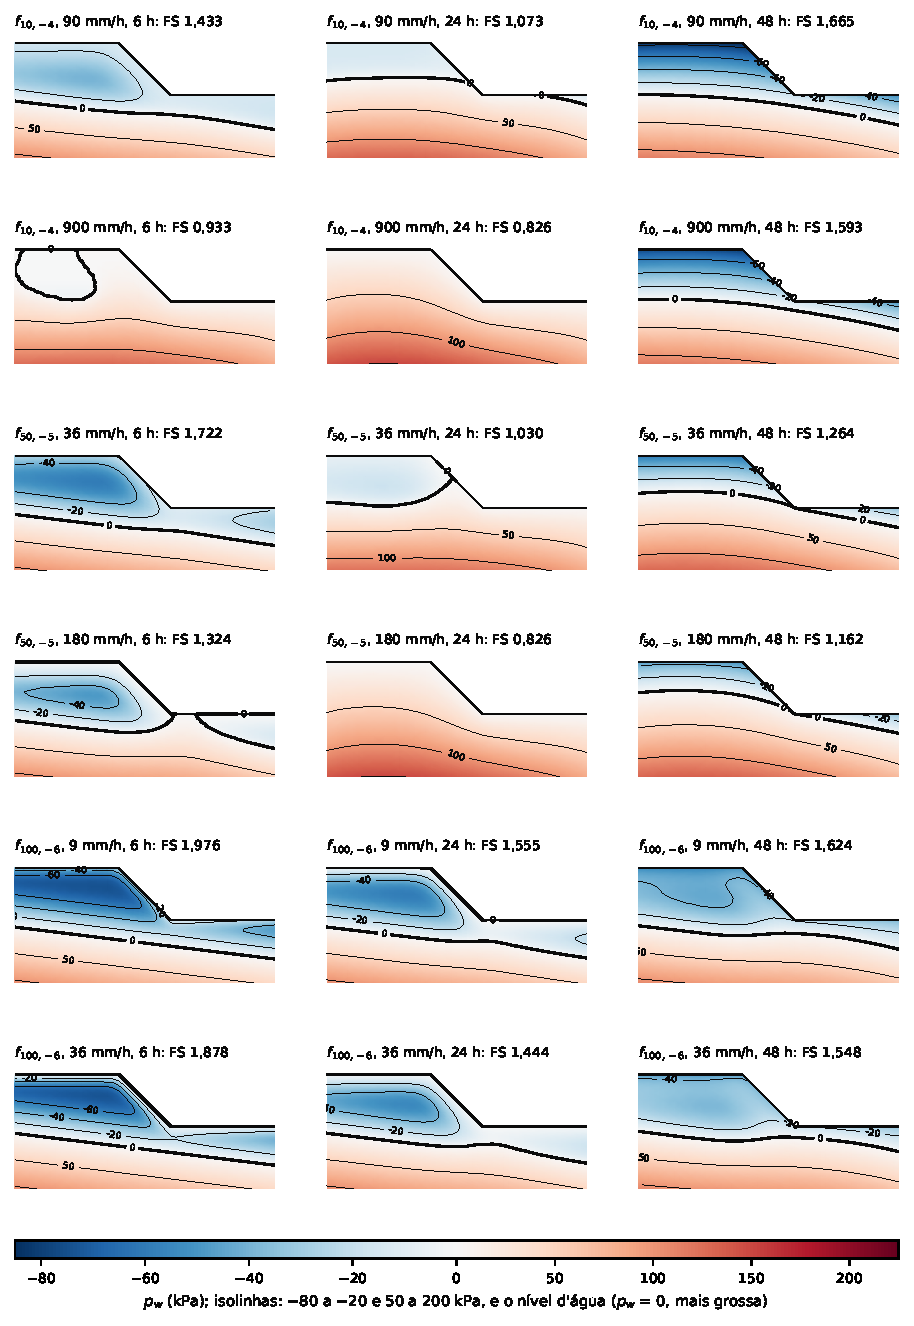
\includegraphics[width=\textwidth]{figs/campos.pdf}
\caption{O campo de $p_w$ em 6, 24 e 48~h. Isolinhas a cada 20~kPa na sucção ($-80$ a $-20$~kPa) e a cada 50~kPa
acima de zero; a linha grossa é o nível d'água ($p_w = 0$). Onde ela não aparece ($f_{10,-4}$ a 900 e $f_{50,-5}$ a
180~mm/h em 24~h), o talude está todo saturado.}\label{fig:campos}
\end{figure}
\fi
\ifnum\nMalhasF>0
\begin{figure}[H]\centering
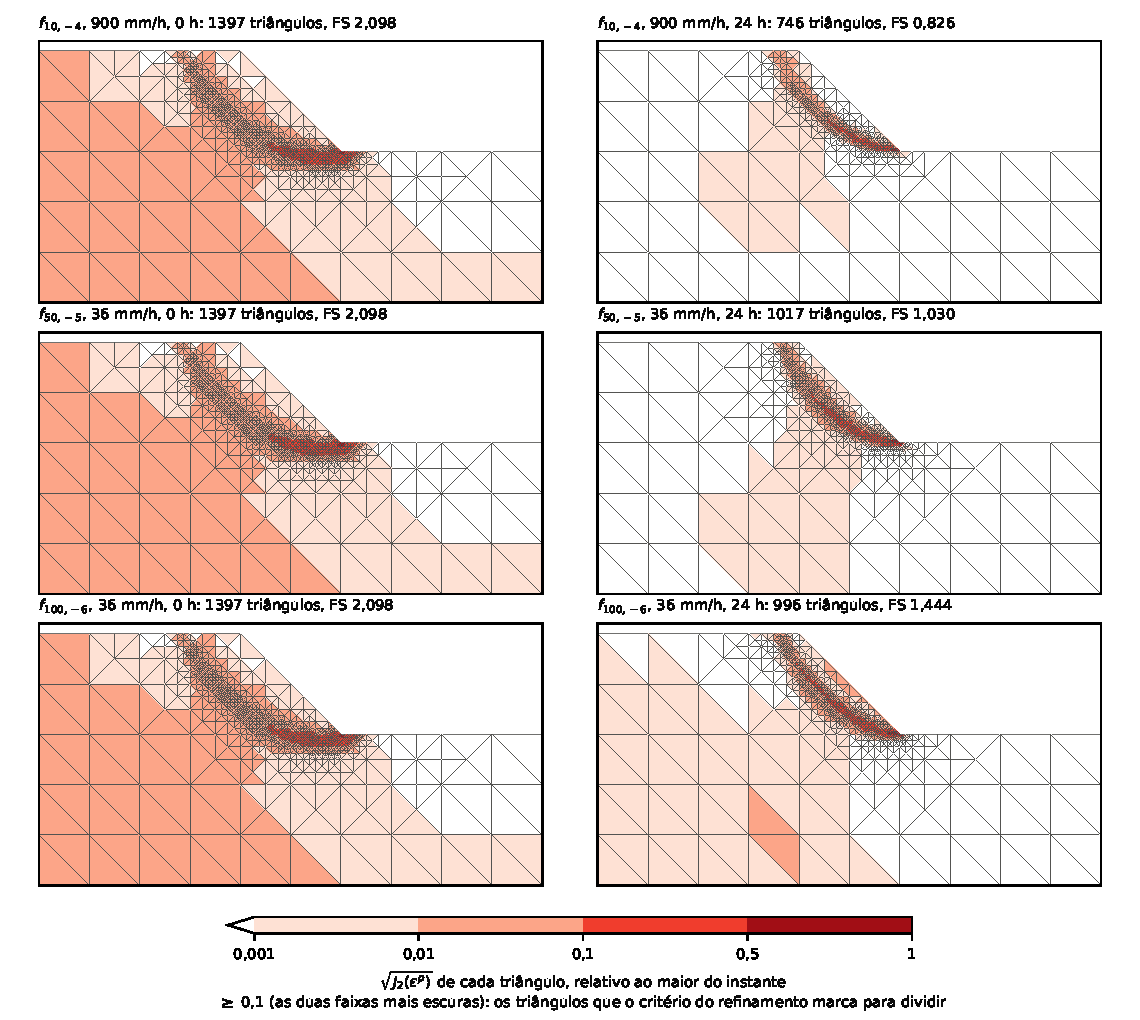
\includegraphics[width=\textwidth]{figs/malhas_fator.pdf}
\caption{A malha final do fator (a malha inicial e 4 níveis adaptativos) em 0 e 24~h, com o indicador plástico
$\sqrt{J_2(\boldsymbol\varepsilon^p)}$ de cada triângulo, relativo ao maior do instante, em faixas de escala log. O
critério do refinamento divide os triângulos com 0,1 ou mais (as duas faixas mais escuras).}\label{fig:malhasF}
\end{figure}
\fi

Os campos mostram o mecanismo por trás das Tabelas~\ref{tab:diag} e \ref{tab:fsmin} (os números abaixo são de $p_w$ numa
vertical sob a crista, $x = 20$~m):
\begin{itemize}
  \item \textbf{$f_{10,-4}$ a 90~mm/h:} em 24~h a camada de cima fica com sucção uniforme de 14~kPa. É a sucção em que
    a permeabilidade iguala a chuva ($k_s\Theta^4 = 90$~mm/h dá $\psi \approx 14$~kPa), o regime de gradiente unitário.
    A sucção não chega a zero e o FS para em 1,07; o nível sobe por baixo até a superfície do pé.
  \item \textbf{$f_{10,-4}$ a 900~mm/h e $f_{50,-5}$ a 180~mm/h:} em 6~h a sucção do $f_{10,-4}$ já foi a zero até
    7~m de profundidade, e em 24~h, nos dois, $p_w > 0$ da superfície à base. A superfície de ruptura fica mais rasa.
    Em 0~h ela sai na crista uns 5~m atrás da quina e passa de 3 a 7~m abaixo do meio da face; em 24~h, no
    $f_{10,-4}$ a 900~mm/h, sai na quina e passa de 2 a 4~m abaixo da face. A malha final do fator cai de 1397 para
    746 triângulos, porque a banda é mais curta (Fig.~\ref{fig:malhasF}).
  \item \textbf{$f_{50,-5}$ a 36~mm/h:} em 24~h a sucção sob a crista cai para 7 a 18~kPa em toda a coluna, e o nível
    sobe 3~m, até a metade de cima da face. A superfície de ruptura sai na crista 1 a 2~m atrás da quina.
  \item \textbf{$f_{100,-6}$:} a frente anda devagar. A 36~mm/h, em 24~h a sucção é zero na superfície e 23~kPa a 2~m,
    mas ainda 51~kPa a 5~m (era 74). O nível não sobe, mas a superfície de ruptura também fica mais rasa: em 24~h ela
    sai na crista 1 a 2~m atrás da quina (era 5~m) e corta a camada molhada junto à face, onde a sucção caiu.
  \item \textbf{Em 48~h}, sem evaporação, a parte de cima drena e a sucção volta. No $f_{10,-4}$ ela passa de 75~kPa
    no topo: é o equilíbrio hidrostático com o nível, sem o limite de 75~kPa do estado inicial. No $f_{100,-6}$ a água
    que entrou se redistribui e a sucção fica em $\approx 45$~kPa nos 5 primeiros metros.
  \item \textbf{A malha do fator} acompanha a banda de cada instante: o refinamento refeito do zero põe os triângulos
    onde a banda está naquele instante, sem herdar a de 0~h.
  \item \textbf{O indicador plástico} (Fig.~\ref{fig:malhasF}) varia ordens de grandeza. No último nível a deformação
    se concentra na face, sobretudo junto ao pé: os triângulos com 0,1 do maior ou mais (os que o critério ainda
    dividiria) ficam entre $x = 30$ e 42~m. A superfície inteira, da crista ao pé, aparece na faixa de 0,01 a 0,1. Em
    0~h, com a resistência dividida por 2,1, a zona atrás da crista também plastifica, com 1 a 10\,\% do maior.
\end{itemize}

\section{Custo computacional}\label{sec:custo}
\begin{table}[H]\centering\small
\caption{Custo por rodada no fermi (Xeon Silver 4116; 7 rodadas por nó, 3 threads cada): os passos e o tempo do
transiente de 48~h, as análises do fator, o tempo por FS (média e mínimo--máximo) e o tempo total (s).}\label{tab:custo}
\resizebox{0.8\textwidth}{!}{\begin{tabular}{lr|cc|ccc|c}
\toprule
 & & \multicolumn{2}{c|}{transiente (48 h)} & \multicolumn{3}{c|}{fator} & \\
solo & $I_r$ & passos & s & análises & s/FS & s/FS (mín--máx) & s total\\
\midrule
$f_{10,-4}$ & 0{,}9 & 480 & 963 & 49 & 62 & 36--81 & 4026\\
$f_{10,-4}$ & 1{,}8 & 480 & 977 & 49 & 62 & 31--78 & 4003\\
$f_{10,-4}$ & 3{,}6 & 480 & 998 & 49 & 58 & 31--78 & 3838\\
$f_{10,-4}$ & 9 & 480 & 1040 & 49 & 56 & 36--77 & 3762\\
$f_{10,-4}$ & 18 & 480 & 1084 & 49 & 51 & 43--77 & 3605\\
$f_{10,-4}$ & 36 & 480 & 1106 & 49 & 48 & 32--77 & 3455\\
$f_{10,-4}$ & 90 & 480 & 1302 & 49 & 43 & 28--77 & 3418\\
$f_{10,-4}$ & 180 & 480 & 1437 & 49 & 36 & 19--77 & 3218\\
$f_{10,-4}$ & 360 & 480 & 1294 & 49 & 33 & 18--77 & 2917\\
$f_{10,-4}$ & 900 & 480 & 1137 & 49 & 34 & 19--77 & 2785\\
$f_{50,-5}$ & 0{,}9 & 480 & 982 & 49 & 60 & 31--78 & 3904\\
$f_{50,-5}$ & 1{,}8 & 480 & 991 & 49 & 58 & 30--78 & 3837\\
$f_{50,-5}$ & 3{,}6 & 480 & 1018 & 49 & 57 & 31--78 & 3801\\
$f_{50,-5}$ & 9 & 480 & 1046 & 49 & 51 & 30--78 & 3529\\
$f_{50,-5}$ & 18 & 480 & 1148 & 49 & 50 & 40--77 & 3583\\
$f_{50,-5}$ & 36 & 480 & 1348 & 49 & 40 & 27--78 & 3301\\
$f_{50,-5}$ & 45 & 480 & 1419 & 49 & 35 & 21--78 & 3157\\
$f_{50,-5}$ & 54 & 480 & 1408 & 49 & 35 & 23--78 & 3135\\
$f_{50,-5}$ & 90 & 480 & 1342 & 49 & 33 & 22--77 & 2983\\
$f_{50,-5}$ & 180 & 480 & 1304 & 49 & 34 & 22--78 & 2948\\
$f_{100,-6}$ & 0{,}36 & 480 & 974 & 49 & 60 & 31--80 & 3905\\
$f_{100,-6}$ & 0{,}9 & 480 & 946 & 49 & 56 & 26--78 & 3672\\
$f_{100,-6}$ & 1{,}8 & 480 & 1023 & 49 & 56 & 30--78 & 3782\\
$f_{100,-6}$ & 3{,}6 & 480 & 1051 & 49 & 54 & 31--78 & 3696\\
$f_{100,-6}$ & 5{,}4 & 480 & 1060 & 49 & 51 & 32--78 & 3584\\
$f_{100,-6}$ & 9 & 480 & 1129 & 49 & 49 & 23--78 & 3527\\
$f_{100,-6}$ & 18 & 480 & 1199 & 49 & 49 & 30--78 & 3587\\
$f_{100,-6}$ & 36 & 480 & 1154 & 49 & 48 & 31--78 & 3501\\
\bottomrule
\end{tabular}
}
\end{table}

Cada rodada (48~h de transiente e 49 FS) levou de \custoMin{} a \custoMax{}~min no fermi (média \custoMedio~min).
As 28 rodadas, em 4 nós, levaram \campanha~min do início ao fim. O FS custa mais que o transiente: 33 a 62~s por
análise, 55 a 76\,\% do total, contra 950 a 1440~s para o transiente inteiro (480 passos). O FS sai mais barato
com o talude perto do colapso, porque o caminho de carga até o patamar é mais curto. O transiente sai mais caro nas
chuvas que alagam a superfície, porque o Newton itera mais com a troca entre fluxo e face de percolação.

\section{O ar ativo: modelo (i)}\label{sec:ar}
\subsection{O que muda}
As mesmas 28 rodadas, com as mesmas malhas, o mesmo passo de tempo, os mesmos instantes do FS e o mesmo SRM, mas com o
transiente completo (as 28 rodadas; a do $f_{100,-6}$ a 5,4~mm/h foi refeita à parte, porque a sua trava ficou vazia na
primeira leva):
\begin{itemize}
  \item \textbf{Acoplamento:} $\mathbf u$, $p_w$ e $p_a$ resolvidos juntos, com o esqueleto elástico ($E = 20$~MPa,
    $\nu = 0{,}3$, os do \texttt{det\_3solos}; o artigo não dá). No transiente o Mohr--Coulomb tem $c' = 10^9$: ele só
    dá as pressões e a deformação. O transiente parte do estado geostático (o peso com as pressões iniciais).
  \item \textbf{O ar:} $p_a$ livre, com $p_a = 0$ só na superfície; na base e nas laterais o fluxo de ar é nulo, e o ar
    só sai por cima. Permeabilidade relativa ao ar de Brooks--Corey ($\lambda = 3$) com piso de $10^{-4}$;
    $\mu_w/\mu_a = 55{,}6$ (com o poro livre e o mesmo gradiente de pressão, o ar anda 55,6 vezes mais que a água);
    ar como gás ideal ($p_{atm} = 101{,}3$~kPa).
  \item \textbf{O fator:} $p_w$ e $p_a$ congeladas. Com $\chi = 1$ a resistência só depende de $\sigma - p_w$, e o ar
    entra no FS pela poropressão: $p_w = p_a - s$. Com a mesma sucção (a mesma umidade), mais ar comprimido quer dizer
    mais $p_w$ e menos resistência.
  \item \textbf{O estado inicial é o mesmo:} o FS em 0~h sai 2,098 nos dois modelos.
\end{itemize}

\subsection{O FS no tempo e a pressão do ar}
\IfFileExists{figs/fs_tempo_i.pdf}{%
\begin{figure}[H]\centering
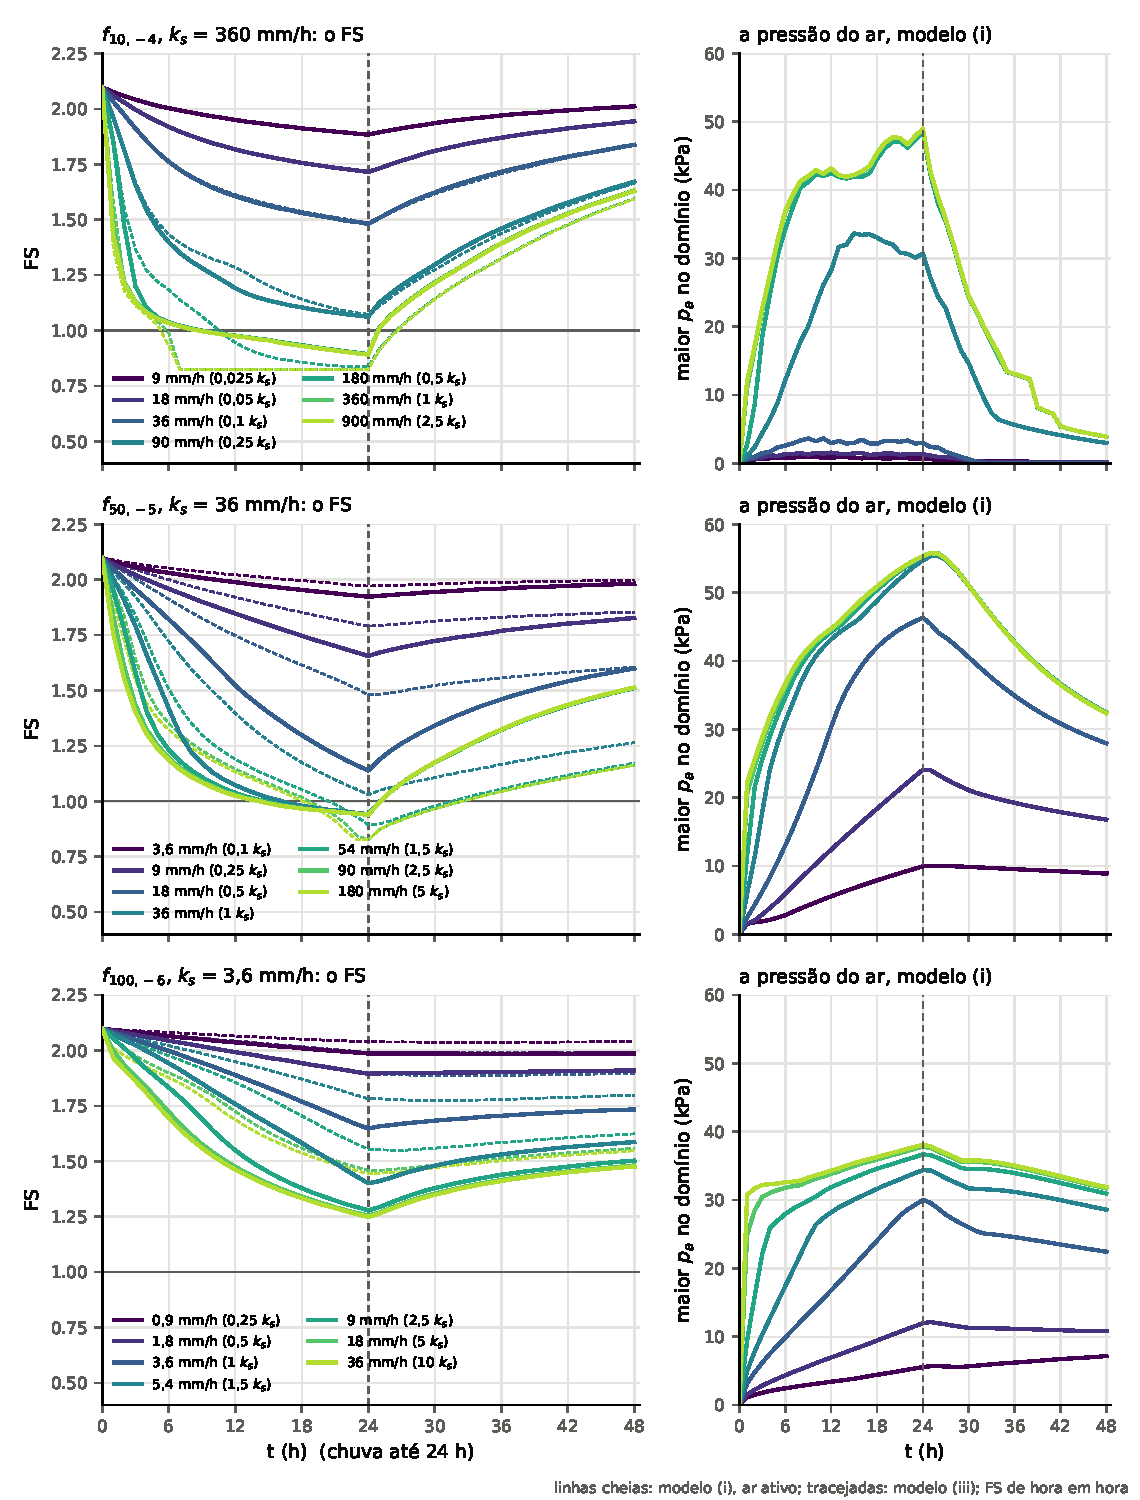
\includegraphics[width=0.92\textwidth]{figs/fs_tempo_i.pdf}
\caption{O FS (à esquerda) nos modelos (i), linhas cheias, e (iii), tracejadas, e a maior pressão do ar no domínio no
(i) (à direita), nas 21 rodadas da Fig.~5. Chuva até 24~h. Nas seis rodadas que gravam campos, a maior $p_a$ fica
sempre na zona não saturada (no $f_{10,-4}$ e no $f_{50,-5}$, logo acima da zona saturada).}\label{fig:fsi}
\end{figure}}{}

\begin{itemize}
  \item \textbf{$f_{10,-4}$:} até 36~mm/h ($k_s/10$) o ar escapa pela superfície. A maior $p_a$ fica abaixo de 4~kPa,
    e o FS é o do (iii) a menos de 0,005. A 90~mm/h, $p_a$ chega a 34~kPa, mas o FS muda só 0,011. De 180~mm/h para
    cima, $p_a$ fica em 49~kPa e o FS para em 0,89, acima do patamar saturado do (iii) (0,83).
  \item \textbf{$f_{50,-5}$:} o ar age em todas as intensidades. A maior $p_a$ vai de 10~kPa (3,6~mm/h) a 55 e 56~kPa
    (36~mm/h ou mais), e o FS cai mais depressa que no (iii). Até 45~mm/h o FS do (i) fica abaixo do (iii); de 54~mm/h para cima, o
    (i) para em 0,94 e o (iii) desce até 0,83 a 0,89.
  \item \textbf{$f_{100,-6}$:} a maior $p_a$ chega a 30~kPa a 3,6~mm/h e a 37--38~kPa de 9~mm/h para cima. O FS do (i) fica
    abaixo do (iii) em todas as intensidades, 0,20 a 0,37 abaixo de 3,6~mm/h para cima, o máximo a 5,4~mm/h
    ($1{,}5\,k_s$).
  \item \textbf{O mínimo cai no fim da chuva:} em \iMinVinte{} das \iFeitos{} rodadas do (i), o FS mínimo é o de 24~h
    (no $f_{100,-6}$ a 0,36 e 0,9~mm/h ele ainda cai devagar até 48 e 34~h). No (iii) o $f_{100,-6}$ até 9~mm/h tinha o
    mínimo depois da chuva, entre 27 e 35~h, porque a água continuava descendo.
  \item \textbf{Depois da chuva:} quando a chuva para, a superfície deixa de receber água, o ar sai e $p_a$ cai. O FS
    do (i) sobe logo: no $f_{10,-4}$ e no $f_{50,-5}$, ele ganha 0,05 a 0,12 na primeira hora. Em 48~h, o $f_{50,-5}$
    está em 1,51 no (i) e em 1,16 a 1,26 no (iii). No $f_{100,-6}$ o ar sai devagar ($p_a$ ainda de 22 a 32~kPa em 48~h,
    de 3,6~mm/h para cima), e o FS do (i) continua abaixo do (iii).
\end{itemize}

\subsection{O FS mínimo e a Eq.~6 com ar}
\IfFileExists{figs/fs_min_i.pdf}{%
\begin{figure}[H]\centering
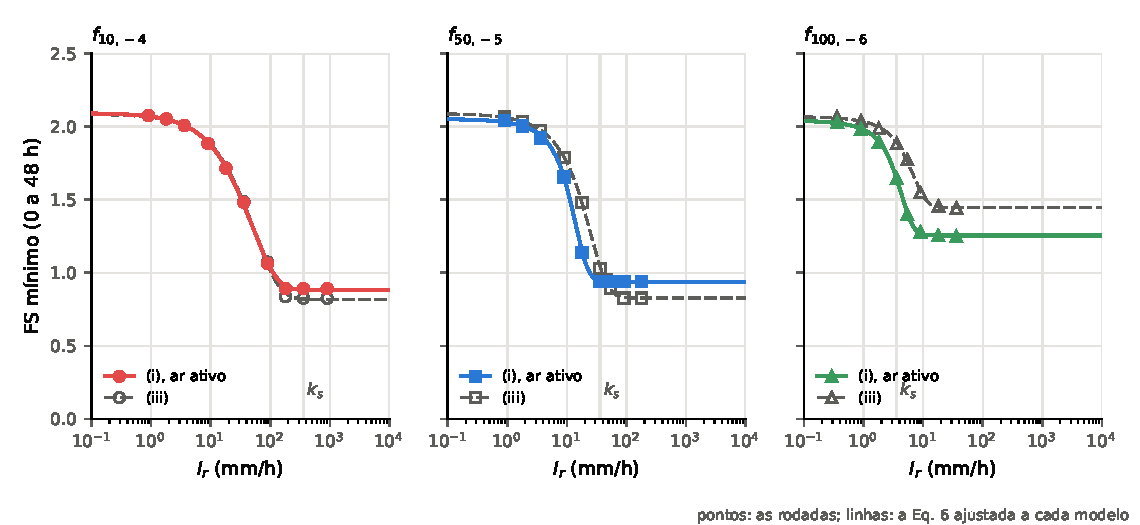
\includegraphics[width=\textwidth]{figs/fs_min_i.pdf}
\caption{O FS mínimo (0 a 48~h) contra a intensidade nos modelos (i) (cheios) e (iii) (vazios), cada um com a sua Eq.~6
ajustada (Tabela~\ref{tab:eq6i}).}\label{fig:fsmini}
\end{figure}}{}

\begin{table}[H]\centering\small
\caption{A Eq.~6, $F_{s(min)} = A + B/\{1 + \exp[-(I_r - C)/D]\}$, ajustada a cada modelo (os parâmetros do (iii) são
os da Tabela~\ref{tab:eq6}). $^\dagger$: $C$ fixo no valor do artigo, nos três modelos. $I_{r(ini)}$ e $I_{r(thr)}$:
a mesma construção da Tabela~\ref{tab:eq6}.}\label{tab:eq6i}
\resizebox{\textwidth}{!}{\begin{tabular}{ll|cccc|c|ccc}
\toprule
solo & modelo & $A$ & $B$ & $C$ & $D$ & $r^2$ & $I_{r(ini)}$ & $I_{r(thr)}$ & $I_{r(thr)}/k_s$\\
 & & & & (mm/h) & (mm/h) & & (mm/h) & (mm/h) & \\
\midrule
$f_{10,-4}$ & (iii), 10 pontos & 0{,}82 & 13{,}92 & -118$^\dagger$ & -51{,}25 & 0{,}999 & 10{,}19 & 144{,}17 & 0{,}40\\
 & (ii), 10 pontos & 0{,}82 & 13{,}71 & -118$^\dagger$ & -51{,}64 & 0{,}999 & 10{,}28 & 145{,}34 & 0{,}40\\
 & (i), 10 pontos & 0{,}88 & 16{,}54 & -118$^\dagger$ & -46{,}46 & 1{,}000 & 9{,}05 & 129{,}81 & 0{,}36\\
\midrule
$f_{50,-5}$ & (iii), 10 pontos & 0{,}83 & 1{,}82 & 10{,}48 & -12{,}77 & 1{,}000 & 7{,}13 & 49{,}07 & 1{,}36\\
 & (ii), 10 pontos & 0{,}87 & 1{,}70 & 11{,}17 & -12{,}29 & 1{,}000 & 7{,}22 & 47{,}95 & 1{,}33\\
 & (i), 10 pontos & 0{,}94 & 1{,}24 & 10{,}39 & -4{,}69 & 1{,}000 & 5{,}66 & 22{,}85 & 0{,}63\\
\midrule
$f_{100,-6}$ & (iii), 8 pontos & 1{,}45 & 0{,}71 & 4{,}87 & -2{,}43 & 0{,}999 & 2{,}63 & 11{,}42 & 3{,}17\\
 & (ii), 8 pontos & 1{,}46 & 0{,}70 & 4{,}92 & -2{,}50 & 0{,}999 & 2{,}66 & 11{,}67 & 3{,}24\\
 & (i), 8 pontos & 1{,}25 & 0{,}86 & 3{,}32 & -1{,}37 & 1{,}000 & 1{,}83 & 6{,}91 & 1{,}92\\
\bottomrule
\end{tabular}
}
\end{table}

\begin{table}[H]\centering\scriptsize\setlength{\tabcolsep}{3pt}
\caption{Cada rodada nos modelos (iii), (ii) e (i): o FS mínimo e a diferença entre (i) e (iii), o instante do mínimo no (i), $t_1$ (o FS cruza 1
descendo; -- se não cruza), a maior $p_a$ do (i), a fração da chuva até 24~h que infiltrou e a hora em que a
superfície começa a alagar.}\label{tab:modeloi}
\resizebox{\textwidth}{!}{\begin{tabular}{lrr|cccc|c|cc|c|cc|cc}
\toprule
 & & & \multicolumn{4}{c|}{FS mínimo (0--48~h)} & instante & \multicolumn{2}{c|}{$t_1$ (h)} & maior $p_a$ & \multicolumn{2}{c|}{infiltrou até 24~h (\%)} & \multicolumn{2}{c}{alaga em (h)}\\
solo & $I_r$ & $I_r/k_s$ & (iii) & (ii) & (i) & (i) $-$ (iii) & do mín. (i) & (iii) & (i) & (i), kPa & (iii) & (i) & (iii) & (i)\\
\midrule
$f_{10,-4}$ & 0{,}9 & 0{,}0025 & 2{,}076 & 2{,}076 & 2{,}075 & 0{,}00 & 24 & -- & -- & 0{,}6 & 100 & 100 & -- & --\\
$f_{10,-4}$ & 1{,}8 & 0{,}005 & 2{,}052 & 2{,}053 & 2{,}052 & 0{,}00 & 24 & -- & -- & 0{,}6 & 100 & 100 & -- & --\\
$f_{10,-4}$ & 3{,}6 & 0{,}01 & 2{,}007 & 2{,}007 & 2{,}007 & 0{,}00 & 24 & -- & -- & 0{,}7 & 100 & 100 & -- & --\\
$f_{10,-4}$ & 9 & 0{,}025 & 1{,}884 & 1{,}885 & 1{,}884 & 0{,}00 & 24 & -- & -- & 1{,}0 & 100 & 100 & -- & --\\
$f_{10,-4}$ & 18 & 0{,}05 & 1{,}716 & 1{,}719 & 1{,}715 & 0{,}00 & 24 & -- & -- & 1{,}6 & 100 & 100 & -- & --\\
$f_{10,-4}$ & 36 & 0{,}1 & 1{,}486 & 1{,}490 & 1{,}481 & 0{,}00 & 24 & -- & -- & 3{,}7 & 100 & 100 & -- & --\\
$f_{10,-4}$ & 90 & 0{,}25 & 1{,}073 & 1{,}076 & 1{,}062 & $-$0{,}01 & 24 & -- & -- & 33{,}7 & 94 & 93 & 14 & 12\\
$f_{10,-4}$ & 180 & 0{,}5 & 0{,}836 & 0{,}837 & 0{,}893 & $+$0{,}06 & 24 & 10{,}55 & 8{,}94 & 48{,}5 & 73 & 61 & 7 & 3\\
$f_{10,-4}$ & 360 & 1 & 0{,}826 & 0{,}826 & 0{,}891 & $+$0{,}07 & 24 & 5{,}80 & 8{,}73 & 48{,}9 & 42 & 31 & 2 & 1\\
$f_{10,-4}$ & 900 & 2{,}5 & 0{,}826 & 0{,}826 & 0{,}891 & $+$0{,}06 & 24 & 5{,}27 & 8{,}67 & 49{,}0 & 17 & 12 & 1 & 1\\
\midrule
$f_{50,-5}$ & 0{,}9 & 0{,}025 & 2{,}064 & 2{,}065 & 2{,}041 & $-$0{,}02 & 24 & -- & -- & 5{,}5 & 100 & 100 & -- & --\\
$f_{50,-5}$ & 1{,}8 & 0{,}05 & 2{,}034 & 2{,}035 & 2{,}003 & $-$0{,}03 & 24 & -- & -- & 6{,}8 & 100 & 100 & -- & --\\
$f_{50,-5}$ & 3{,}6 & 0{,}1 & 1{,}971 & 1{,}974 & 1{,}923 & $-$0{,}05 & 24 & -- & -- & 10{,}0 & 100 & 100 & -- & --\\
$f_{50,-5}$ & 9 & 0{,}25 & 1{,}790 & 1{,}797 & 1{,}656 & $-$0{,}13 & 24 & -- & -- & 24{,}1 & 100 & 100 & -- & --\\
$f_{50,-5}$ & 18 & 0{,}5 & 1{,}480 & 1{,}504 & 1{,}139 & $-$0{,}34 & 24 & -- & -- & 46{,}3 & 100 & 94 & -- & 12\\
$f_{50,-5}$ & 36 & 1 & 1{,}030 & 1{,}052 & 0{,}942 & $-$0{,}09 & 24 & -- & 16{,}25 & 55{,}4 & 87 & 59 & 12 & 4\\
$f_{50,-5}$ & 45 & 1{,}25 & 0{,}951 & 0{,}983 & 0{,}940 & $-$0{,}01 & 24 & 21{,}94 & 15{,}23 & 55{,}7 & 78 & 47 & 9 & 3\\
$f_{50,-5}$ & 54 & 1{,}5 & 0{,}894 & 0{,}942 & 0{,}939 & $+$0{,}05 & 24 & 20{,}42 & 14{,}79 & 55{,}8 & 68 & 40 & 6 & 2\\
$f_{50,-5}$ & 90 & 2{,}5 & 0{,}826 & 0{,}881 & 0{,}939 & $+$0{,}11 & 24 & 18{,}68 & 14{,}28 & 55{,}8 & 42 & 24 & 2 & 1\\
$f_{50,-5}$ & 180 & 5 & 0{,}826 & 0{,}859 & 0{,}940 & $+$0{,}11 & 24 & 18{,}13 & 14{,}22 & 55{,}8 & 21 & 12 & 1 & 1\\
\midrule
$f_{100,-6}$ & 0{,}36 & 0{,}1 & 2{,}065 & 2{,}067 & 2{,}029 & $-$0{,}04 & 48 & -- & -- & 5{,}9 & 100 & 100 & -- & --\\
$f_{100,-6}$ & 0{,}9 & 0{,}25 & 2{,}036 & 2{,}038 & 1{,}984 & $-$0{,}05 & 34 & -- & -- & 7{,}2 & 100 & 100 & -- & --\\
$f_{100,-6}$ & 1{,}8 & 0{,}5 & 1{,}989 & 1{,}992 & 1{,}895 & $-$0{,}09 & 24 & -- & -- & 12{,}2 & 100 & 100 & -- & --\\
$f_{100,-6}$ & 3{,}6 & 1 & 1{,}886 & 1{,}894 & 1{,}648 & $-$0{,}24 & 24 & -- & -- & 30{,}0 & 100 & 100 & -- & 21\\
$f_{100,-6}$ & 5{,}4 & 1{,}5 & 1{,}773 & 1{,}784 & 1{,}401 & $-$0{,}37 & 24 & -- & -- & 34{,}4 & 100 & 93 & -- & 10\\
$f_{100,-6}$ & 9 & 2{,}5 & 1{,}549 & 1{,}565 & 1{,}278 & $-$0{,}27 & 24 & -- & -- & 36{,}7 & 95 & 65 & 11 & 4\\
$f_{100,-6}$ & 18 & 5 & 1{,}458 & 1{,}469 & 1{,}254 & $-$0{,}20 & 24 & -- & -- & 37{,}8 & 56 & 34 & 3 & 1\\
$f_{100,-6}$ & 36 & 10 & 1{,}444 & 1{,}454 & 1{,}249 & $-$0{,}19 & 24 & -- & -- & 38{,}1 & 29 & 17 & 1 & 1\\
\bottomrule
\end{tabular}
}
\end{table}

\begin{itemize}
  \item \textbf{A forma da Eq.~6 continua valendo:} a sigmoide ajusta os pontos do (i) tão bem quanto os do (iii)
    ($r^2 \ge 0{,}999$ nos três solos). O que muda são os parâmetros.
  \item \textbf{O patamar de baixo, $A$,} sobe onde o (iii) satura o talude: de \ATresDez{} para \AUmDez{} no
    $f_{10,-4}$ e de \ATresCinq{} para \AUmCinq{} no $f_{50,-5}$. O ar preso não deixa o solo saturar. No $f_{100,-6}$,
    onde o nível não chega à superfície nem no (iii), $A$ cai de \ATresCem{} para \AUmCem: ali o ar comprimido levanta
    $p_w$ em toda a zona molhada.
  \item \textbf{A transição vai para chuvas menores e fica mais abrupta:} $I_{r(thr)}$ cai de \ThrTresDez{} para
    \ThrUmDez~mm/h no $f_{10,-4}$ (de \ThrksTresDez{} para \ThrksUmDez~$k_s$), de \ThrTresCinq{} para \ThrUmCinq{}
    (\ThrksTresCinq{} para \ThrksUmCinq~$k_s$) no $f_{50,-5}$ e de \ThrTresCem{} para \ThrUmCem{} (\ThrksTresCem{} para
    \ThrksUmCem~$k_s$) no $f_{100,-6}$. $I_{r(ini)}$ cai de \IniTresDez{} para \IniUmDez, de \IniTresCinq{} para
    \IniUmCinq{} e de \IniTresCem{} para \IniUmCem~mm/h. $|D|$, a largura da transição, cai de \DTresDez{} para
    \DUmDez, de \DTresCinq{} para \DUmCinq{} e de \DTresCem{} para \DUmCem~mm/h.
  \item \textbf{As curvas se cruzam} no $f_{10,-4}$ (perto de 100~mm/h) e no $f_{50,-5}$ (entre 45 e 54~mm/h). Abaixo
    do cruzamento o ar baixa o FS mínimo; acima, sobe. No $f_{100,-6}$ elas não se cruzam: o ar baixa o FS mínimo em
    todas as intensidades.
  \item \textbf{As maiores quedas} são de \quedaCem{} no $f_{100,-6}$ a \quedaCemI~mm/h ($1{,}5\,k_s$: FS mínimo de
    1,40 contra 1,77) e de \quedaCinq{} no $f_{50,-5}$ a \quedaCinqI~mm/h ($k_s/2$: 1,14 contra 1,48), as duas logo
    abaixo da intensidade em que o (iii) começa a alagar a superfície. No $f_{50,-5}$ a 36~mm/h o (i) rompe ($t_1$ =
    16,3~h) e o (iii) não (FS mínimo de 1,03).
\end{itemize}

\subsection{A deformação sem o ar: modelo (ii)}\label{sec:modeloii}
O modelo (ii) é o (iii) com o esqueleto elástico acoplado ($E = 20$~MPa, $\nu = 0{,}3$, o mesmo do (i)), sem a fase de
ar ($p_a = 0$). As \iiFeitos{} rodadas separam o que o (i) muda em duas partes: a deformação, (ii) $-$ (iii), e o ar,
(i) $-$ (ii).

\IfFileExists{figs/decomposicao.pdf}{%
\begin{figure}[H]\centering
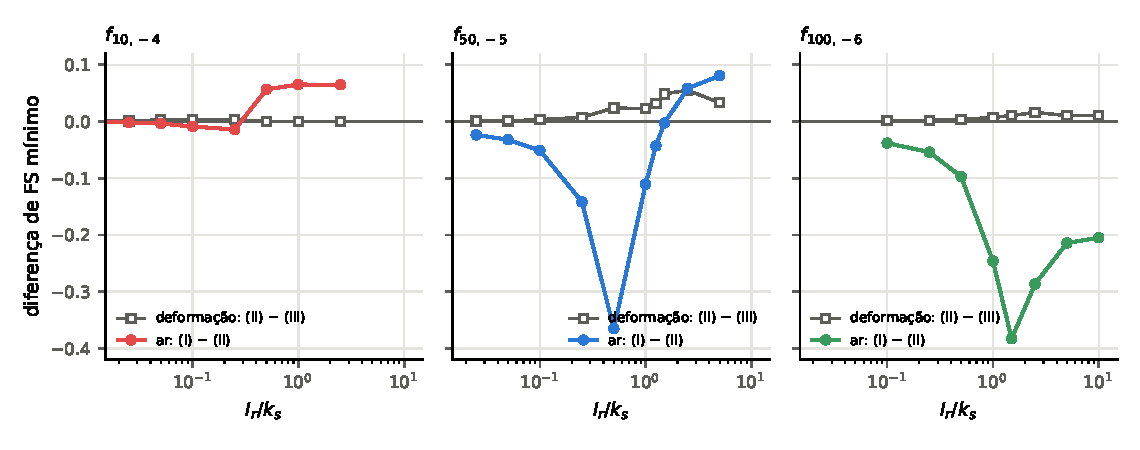
\includegraphics[width=\textwidth]{figs/decomposicao.pdf}
\caption{A diferença de FS mínimo separada em deformação, (ii) $-$ (iii), e ar, (i) $-$ (ii), contra a intensidade em
múltiplos de $k_s$.}\label{fig:decomp}
\end{figure}}{}

\begin{itemize}
  \item \textbf{O FS em 0~h é o mesmo} (2,098): o estado geostático não muda as pressões.
  \item \textbf{A deformação pesa pouco:} ela muda o FS mínimo de 0 a $+$\defMax{} (o maior no \defMaxSolo{} a
    \defMaxI~mm/h). O esqueleto que se deforma guarda um pouco mais de água, e a poropressão sobe um pouco mais devagar.
    Nas chuvas fortes do $f_{50,-5}$, em 24~h o (ii) ainda não chegou ao patamar saturado (0,86 a 0,88, contra 0,83); no
    $f_{10,-4}$ a 360 e 900~mm/h ele chega ao mesmo 0,826, só uma a duas horas depois (9 a 10~h, contra 7 a 8~h).
  \item \textbf{O ar explica quase tudo:} a diferença (i) $-$ (ii) vai de $-$\arMin{} (\arMinSolo{} a \arMinI~mm/h) a
    $+$\arMax{} (\arMaxSolo{} a \arMaxI~mm/h), praticamente a mesma (i) $-$ (iii) da Tabela~\ref{tab:modeloi}.
  \item \textbf{Na Eq.~6} (Tabela~\ref{tab:eq6i}) os parâmetros do (ii) ficam perto dos do (iii): $I_{r(thr)}$ de
    \ThrksDoisDez, \ThrksDoisCinq{} e \ThrksDoisCem~$k_s$, contra \ThrksTresDez, \ThrksTresCinq{} e \ThrksTresCem. O
    patamar $A$ do $f_{50,-5}$ sobe de \ATresCinq{} para \ADoisCinq{} porque, em 24~h, o (ii) ainda não saturou.
  \item \textbf{Consequência:} a correção da Eq.~6 é do ar. Para ela, tanto faz tomar como referência o (iii) (o SEEP/W
    do artigo) ou o (ii).
\end{itemize}

\subsection{O mecanismo: os campos de pressão}\label{sec:campos_i}
\ifnum\nCamposI>0
\begin{figure}[H]\centering
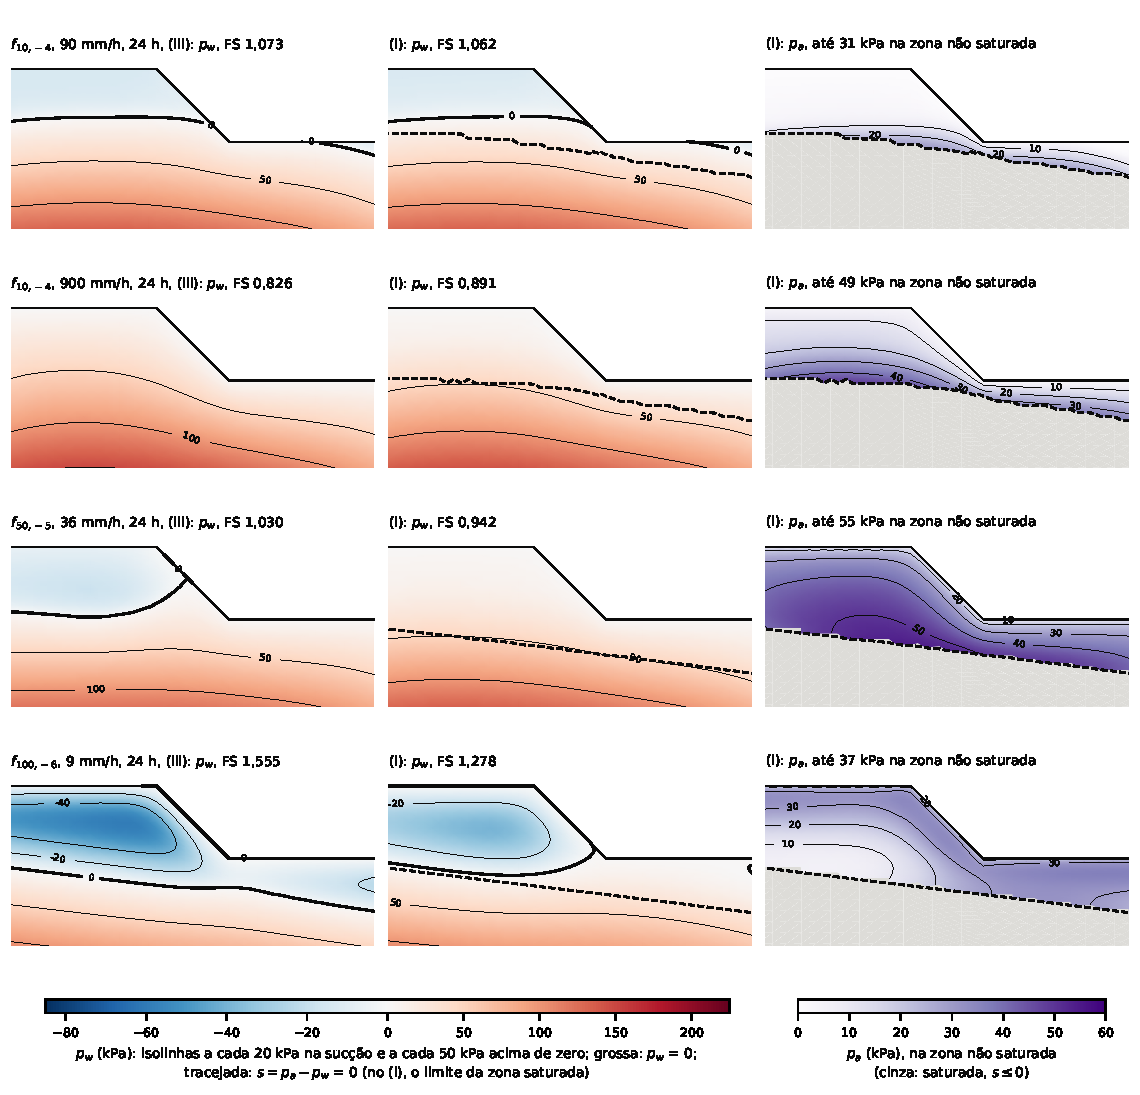
\includegraphics[width=\textwidth]{figs/campos_i.pdf}
\caption{Os campos em 24~h, o instante do FS mínimo do (i): $p_w$ no (iii), $p_w$ no (i) e $p_a$ no (i), em quatro das
seis rodadas que gravam campos. A linha grossa é $p_w = 0$; a tracejada, $s = p_a - p_w = 0$. No (iii) a zona saturada
é $p_w \ge 0$; no (i) ela é $s \le 0$ (abaixo da tracejada, e em cinza no painel de $p_a$).}\label{fig:camposi}
\end{figure}
\fi

Os números abaixo são de uma vertical sob a crista ($x = 20$~m), em 24~h:
\begin{itemize}
  \item \textbf{$f_{50,-5}$ a 36~mm/h, o ar levanta $p_w$:} no (i), $p_w > 0$ desde a superfície (0,3~kPa a 5~cm,
    5~kPa a 2~m, 11~kPa a 5~m), mas o solo ainda tem de 8 a 32~kPa de sucção. É $p_a$, de 8~kPa na superfície a
    50~kPa a 10~m, que empurra a água. No (iii), $p_w$ fica entre $-7$ e $-18$~kPa nos 8~m de cima. A poropressão sobe de
    7~kPa (na superfície) a 28~kPa (a 5~m), e o FS cai de 1,03 para 0,94. É o mesmo efeito dos poços em que o nível
    d'água sobe de repente numa chuva forte (o efeito Lisse): o ar preso entre a frente de umedecimento e o nível d'água
    é comprimido e empurra a água.
  \item \textbf{No (i), $p_w = 0$ deixa de marcar a zona saturada.} O limite da zona saturada é $s = 0$ (tracejada). No
    $f_{50,-5}$ a 36~mm/h, a linha $p_w = 0$ já saiu pela crista em 24~h, mas o solo acima da tracejada ainda não está
    saturado. Por isso as rodadas do (i) não são classificadas pelas categorias da Tabela~3: pela linha $p_w = 0$, o
    $f_{50,-5}$ já seria I a 36~mm/h e o $f_{100,-6}$ seria III de 9~mm/h para cima, com o solo ainda com sucção.
  \item \textbf{$f_{10,-4}$ a 900~mm/h, o ar segura a saturação:} no (iii) o talude está todo saturado, com percolação
    ($p_w$ = 11~kPa a 2~m e 59~kPa a 10~m). No (i) o ar preso mantém de 2 a 5~kPa de sucção nos 10~m de cima, e $p_w$
    fica menor (5,6 e 46~kPa). O FS fica em 0,89, contra 0,83. Entra menos água (12\,\% da chuva, contra 17\,\%).
  \item \textbf{$f_{100,-6}$ a 9~mm/h:} no (i), $p_a$ de 10 a 31~kPa nos 5~m de cima, e $p_w$ de 4 a 20~kPa maior que no
    (iii) ($-18$ contra $-35$~kPa a 2~m; $-37$ contra $-57$~kPa a 5~m). O FS cai de 1,55 para 1,28.
  \item \textbf{$f_{10,-4}$ a 90~mm/h, o ar escapa:} $p_a$ fica abaixo de 3,5~kPa nos 6~m de cima, e $p_w$ é a do (iii) a
    menos de 2~kPa. O FS é praticamente o mesmo (1,062 contra 1,073).
  \item \textbf{A superfície de ruptura é a mesma:} nas seis rodadas, as malhas do fator em 24~h põem a banda no mesmo
    lugar nos dois modelos. Ela sai na crista em $x$ = 27,3 a 27,9~m e passa de 2 a 4,5~m abaixo do meio da face. O ar
    muda o FS pela pressão, não pelo mecanismo.
\end{itemize}

\subsection{Linhas de controle: $p_w$, a sua taxa de variação, $p_a$ e a saturação}\label{sec:perfis}
Duas verticais de controle, uma sob a crista ($x = 20$~m) e outra no meio da face ($x = 35$~m), com $p_w$ contra a
profundidade nos instantes em que as rodadas gravam o campo (0, 6, 12, 24 e 48~h). A taxa de variação é a média entre
dois desses instantes, $[p_w(t_2) - p_w(t_1)]/(t_2 - t_1)$. Uma série de hora em hora num ponto exigiria gravar $p_w$
em cada passo, o que as rodadas não fizeram.

\ifnum\nPerfis>0
\begin{figure}[H]\centering
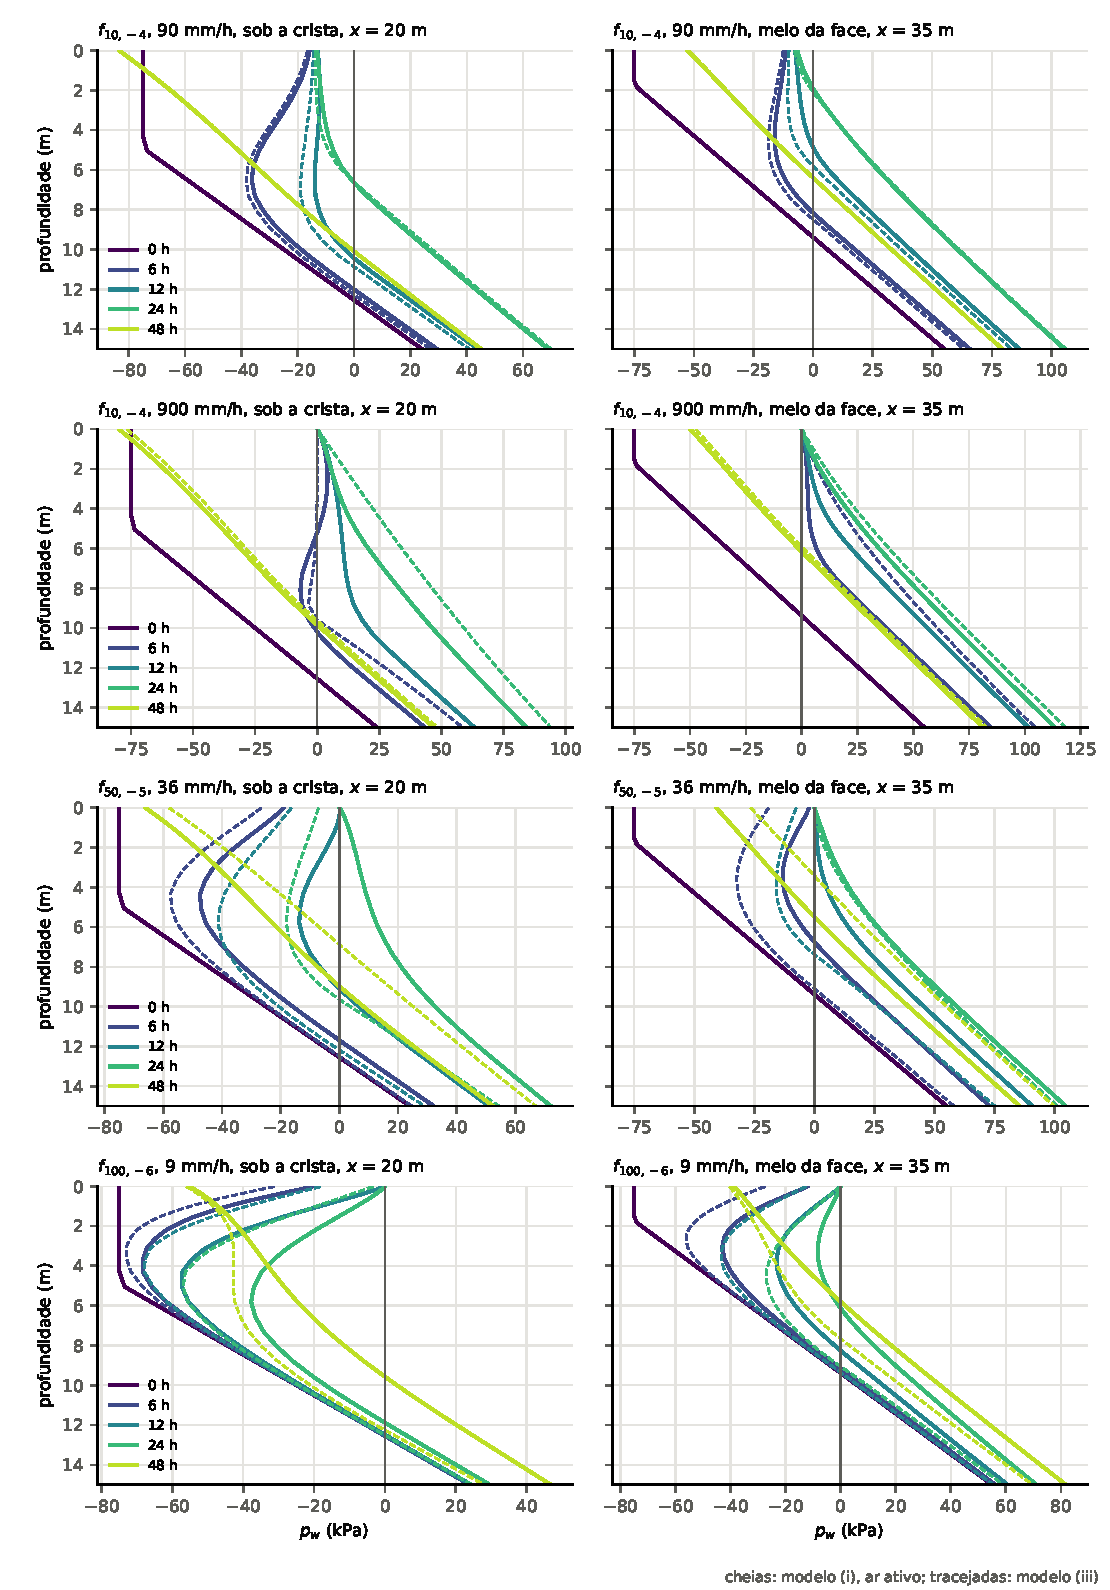
\includegraphics[width=0.92\textwidth]{figs/perfis_i.pdf}
\caption{$p_w$ nas duas verticais de controle, nos modelos (i) (cheias) e (iii) (tracejadas), em 0, 6, 12, 24 e 48~h.}
\label{fig:perfis}
\end{figure}
\begin{figure}[H]\centering
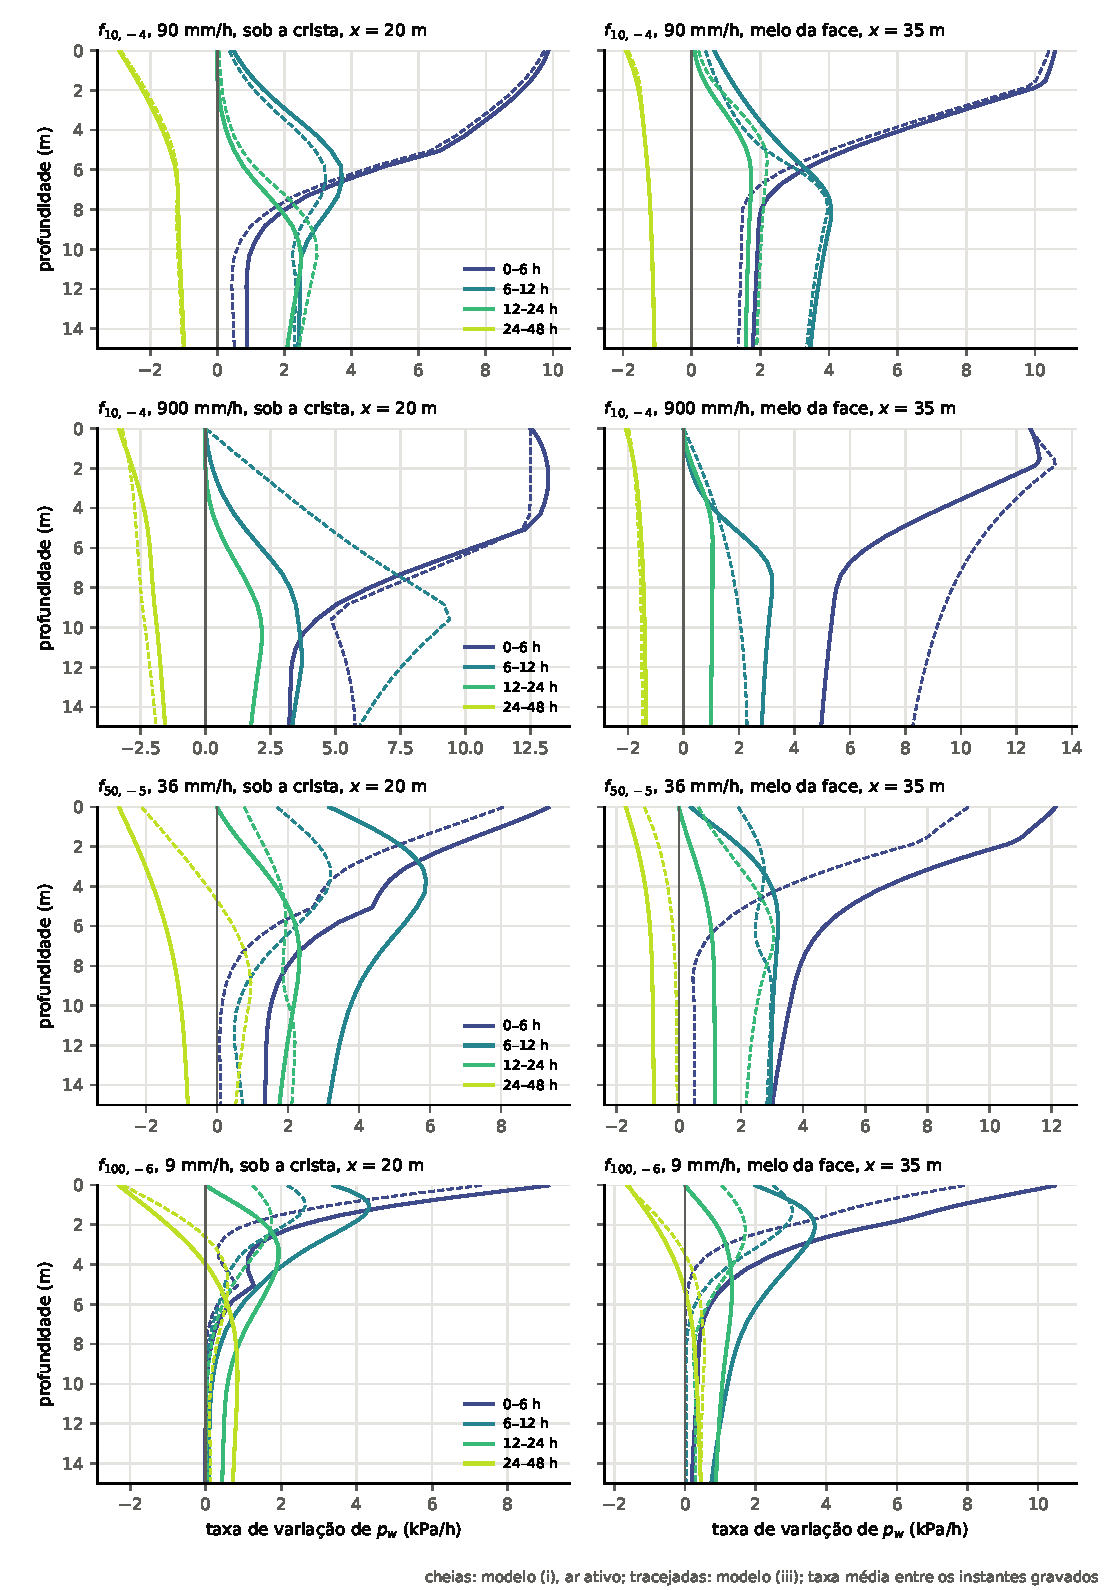
\includegraphics[width=0.92\textwidth]{figs/taxa_i.pdf}
\caption{A taxa média de variação de $p_w$ (kPa/h) nas mesmas verticais, entre os instantes gravados: 0--6, 6--12,
12--24 e 24--48~h.}\label{fig:taxa}
\end{figure}
\begin{figure}[H]\centering
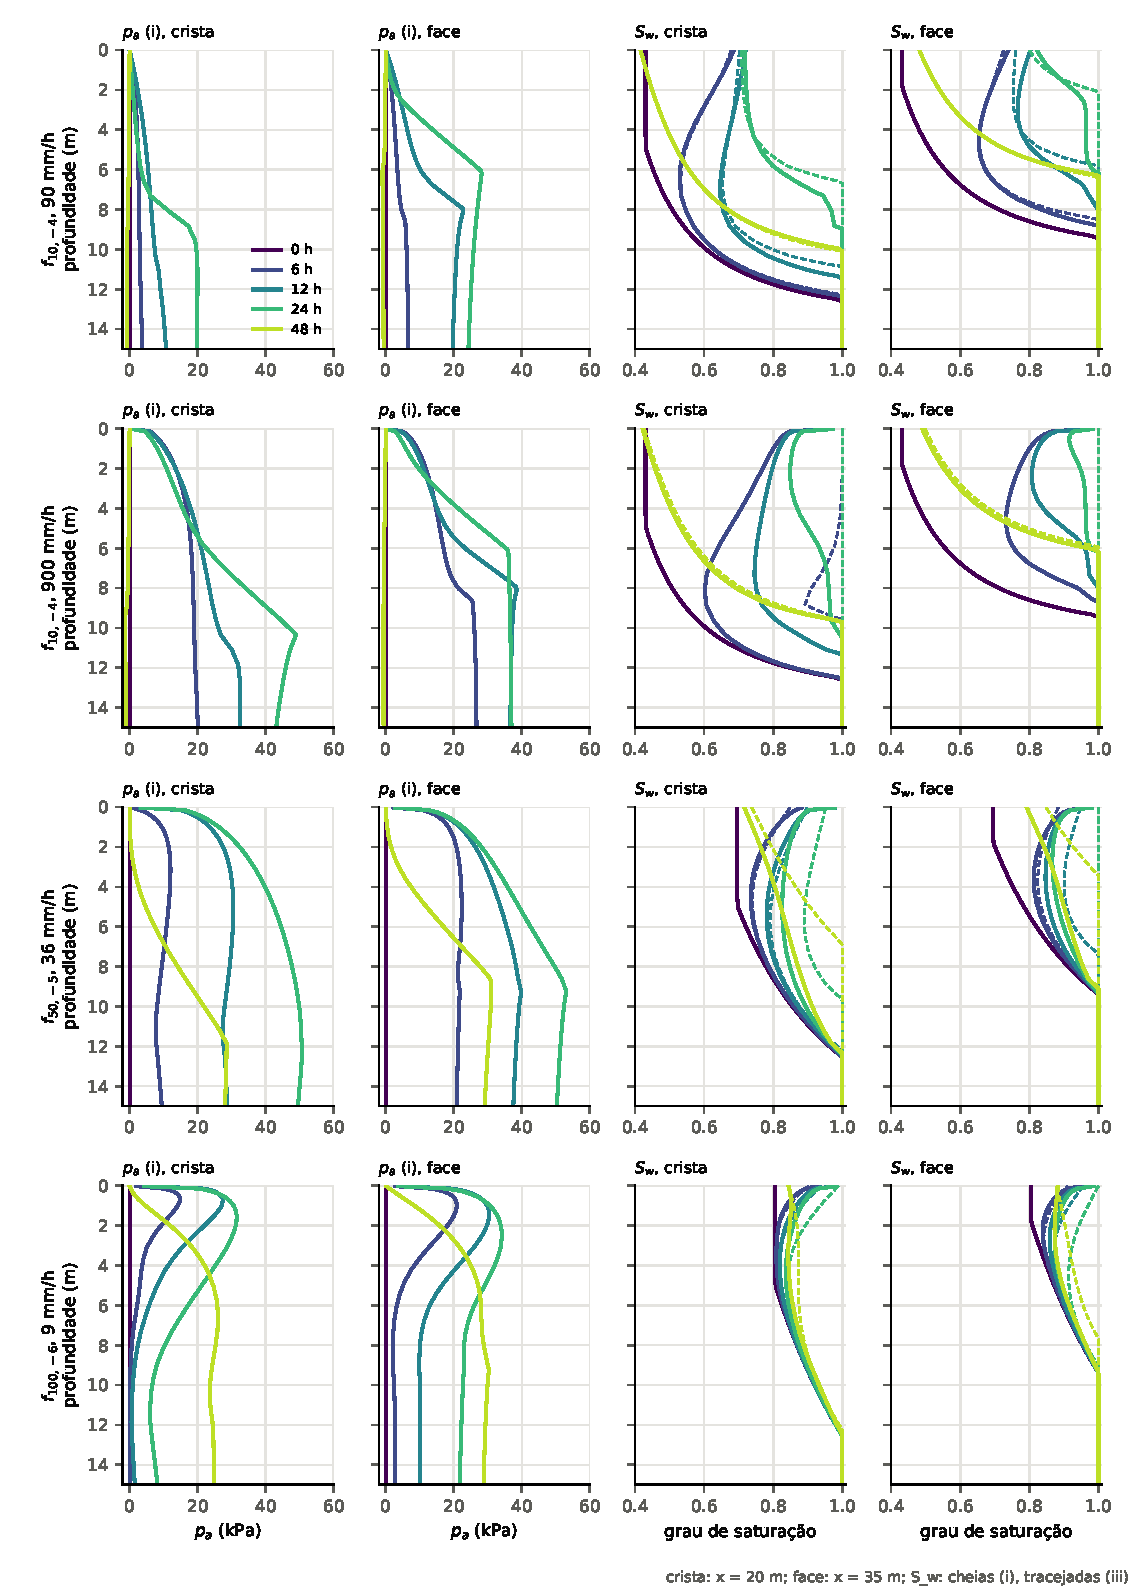
\includegraphics[width=\textwidth]{figs/perfis_ar_i.pdf}
\caption{Nas mesmas verticais e instantes: a pressão do ar no (i) e o grau de saturação nos dois modelos ((i) cheias,
(iii) tracejadas). $S_w$ vem da curva de retenção com a sucção $s = p_a - p_w$ ($s = -p_w$ no (iii)):
$S_w = 1/\ln(e + s/a)$ para $s > 0$ e 1 para $s \le 0$.}\label{fig:perfisar}
\end{figure}
\fi

\begin{itemize}
  \item \textbf{No (iii), $p_w$ só sobe onde a frente chega.} Abaixo dela, a taxa fica perto de zero. No $f_{50,-5}$ a
    36~mm/h, sob a crista a 10~m, ela é 0,1~kPa/h de 0 a 6~h e 0,6~kPa/h de 6 a 12~h.
  \item \textbf{No (i), $p_w$ sobe também à frente da frente,} porque o ar comprimido transmite a pressão: no mesmo
    ponto, 1,5 e 3,8~kPa/h. No $f_{100,-6}$ a 9~mm/h, a 6~m, 0,6 e 0,9~kPa/h contra 0,3 e 0,3. Por isso no (i) toda a
    coluna perde sucção ao mesmo tempo, e não só a camada molhada.
  \item \textbf{Perto da superfície,} o (i) sobe mais depressa no começo ($f_{50,-5}$ a 36~mm/h, a 1~m sob a crista:
    8,0 contra 6,5~kPa/h de 0 a 6~h) e depois quase para (0,4 contra 1,1 de 12 a 24~h). O ar já levou $p_w$ para
    perto do valor em que a sucção que sobra segura a água.
  \item \textbf{$f_{10,-4}$ a 900~mm/h:} no (iii) $p_w$ para de mudar depois de 12~h (o regime permanente saturado,
    taxa zero de 12 a 24~h). No (i) ela continua subindo devagar (1 a 2~kPa/h abaixo de 6~m de 12 a 24~h), porque o
    ar preso sai aos poucos.
  \item \textbf{$f_{10,-4}$ a 90~mm/h:} as taxas dos dois modelos ficam a menos de 0,6~kPa/h uma da outra: o ar escapa.
  \item \textbf{Mais pressão com menos água} (Fig.~\ref{fig:perfisar}, em 24~h): no (i) o solo fica \emph{menos}
    saturado que no (iii) e, mesmo assim, com $p_w$ maior. No $f_{50,-5}$ a 36~mm/h, sob a crista, $S_w$ é 0,86, 0,83
    e 0,83 a 1, 3 e 6~m, contra 0,94, 0,91 e 0,89 no (iii), com $p_a$ de 27, 37 e 45~kPa. No meio da face o (iii) já
    está saturado ($S_w = 1$) até 10~m, e o (i) fica entre 0,87 e 0,90. No $f_{10,-4}$ a 900~mm/h o (iii) está todo
    saturado, e o (i) fica com $S_w$ de 0,85 a 0,98 nos 10~m de cima. É o ar que ocupa os poros e não deixa a água
    entrar, e é a sua pressão que empurra $p_w$ para cima.
  \item \textbf{O perfil de $p_a$} cresce com a profundidade até perto da zona saturada: o ar sai pela superfície e
    fica preso por baixo. Ele chega a 45--52~kPa a 6--10~m no $f_{50,-5}$ a 36~mm/h. No $f_{100,-6}$ a 9~mm/h o máximo
    (cerca de 30~kPa) fica a 1--3~m, logo abaixo da frente, e cai mais fundo. No $f_{10,-4}$ a 90~mm/h, $p_a$ fica em
    0 a 3~kPa nos 6~m de cima.
  \item \textbf{Depois da chuva (24--48~h)} as taxas ficam negativas na parte de cima nos dois modelos (a drenagem). No
    (i) a queda é um pouco maior, porque $p_a$ também cai.
\end{itemize}

\subsection{A duração da chuva}\label{sec:duracao}
O artigo usa 24~h em todas as séries. Com a chuva constante desde $t = 0$, uma chuva de $D \le 24$~h tem a mesma
história da de 24~h até $t = D$. Então o FS em $t = D$ das nossas rodadas é o FS no fim de uma chuva de duração $D$.
Ele é um limite de cima do FS mínimo dessa chuva: o mínimo pode vir depois que ela para. Em 24~h, a diferença entre o
FS no fim da chuva e o mínimo de 0 a 48~h é no máximo \durErro{} (no $f_{100,-6}$, onde a água continua descendo). No
(i) o FS sobe logo que a chuva para, e a aproximação deve valer também para chuvas curtas. Para o (iii) e chuvas curtas
ela ainda precisa de rodadas com $D < 24$~h. Chuvas de mais de 24~h precisam de rodadas novas: a etapa 2 no fermi
roda os 28 casos nos dois modelos com chuvas de 6, 12, 48, 72 e 144~h, com o FS até 24~h depois do fim de cada uma.

\IfFileExists{figs/duracao.pdf}{%
\begin{figure}[H]\centering
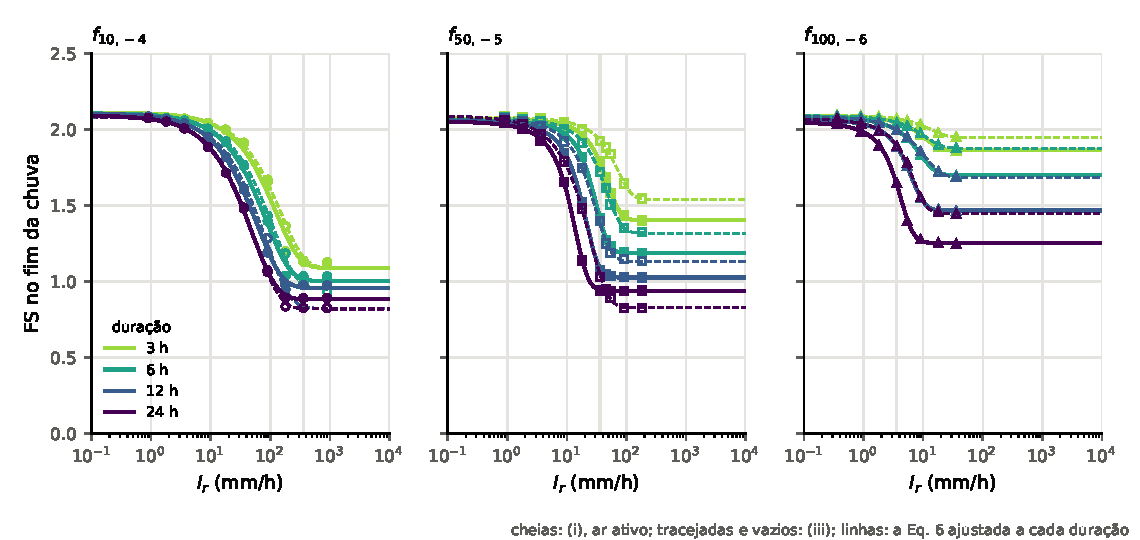
\includegraphics[width=\textwidth]{figs/duracao.pdf}
\caption{O FS no fim de chuvas de 3, 6, 12 e 24~h contra a intensidade (a Fig.~\ref{fig:fsmini} para outras
durações), nos modelos (i) (cheios) e (iii) (vazios, tracejadas), cada curva com a sua Eq.~6.}\label{fig:duracao}
\end{figure}}{}

\begin{table}[H]\centering\small
\caption{Os parâmetros da Eq.~6 ajustada ao FS no fim da chuva, para cada duração: o patamar de baixo $A$ e as
intensidades de início e de limiar em múltiplos de $k_s$.}\label{tab:duracao}
\begin{tabular}{l|cc|cc|cc|cc}
\toprule
 & \multicolumn{8}{c}{duração da chuva}\\
solo, grandeza & \multicolumn{2}{c|}{3 h} & \multicolumn{2}{c|}{6 h} & \multicolumn{2}{c|}{12 h} & \multicolumn{2}{c}{24 h}\\
 & (iii) & (i) & (iii) & (i) & (iii) & (i) & (iii) & (i)\\
\midrule
$f_{10,-4}$, $A$ & 1{,}09 & 1{,}09 & 0{,}95 & 1{,}00 & 0{,}82 & 0{,}96 & 0{,}82 & 0{,}88\\
$f_{10,-4}$, $I_{r(thr)}/k_s$ & 1{,}02 & 0{,}86 & 0{,}76 & 0{,}60 & 0{,}59 & 0{,}43 & 0{,}40 & 0{,}36\\
$f_{10,-4}$, $I_{r(ini)}/k_s$ & 0{,}08 & 0{,}07 & 0{,}06 & 0{,}05 & 0{,}04 & 0{,}03 & 0{,}03 & 0{,}03\\
\midrule
$f_{50,-5}$, $A$ & 1{,}54 & 1{,}40 & 1{,}32 & 1{,}19 & 1{,}13 & 1{,}03 & 0{,}83 & 0{,}94\\
$f_{50,-5}$, $I_{r(thr)}/k_s$ & 3{,}45 & 2{,}21 & 2{,}29 & 1{,}38 & 1{,}52 & 0{,}96 & 1{,}36 & 0{,}63\\
$f_{50,-5}$, $I_{r(ini)}/k_s$ & 0{,}74 & 0{,}56 & 0{,}47 & 0{,}38 & 0{,}30 & 0{,}24 & 0{,}20 & 0{,}16\\
\midrule
$f_{100,-6}$, $A$ & 1{,}95 & 1{,}86 & 1{,}88 & 1{,}70 & 1{,}69 & 1{,}47 & 1{,}45 & 1{,}25\\
$f_{100,-6}$, $I_{r(thr)}/k_s$ & 7{,}27 & 5{,}30 & 5{,}83 & 4{,}58 & 5{,}57 & 2{,}97 & 3{,}23 & 1{,}93\\
$f_{100,-6}$, $I_{r(ini)}/k_s$ & 1{,}16 & 1{,}01 & 0{,}92 & 0{,}85 & 0{,}85 & 0{,}72 & 0{,}75 & 0{,}50\\
\bottomrule
\end{tabular}

\end{table}

\begin{itemize}
  \item \textbf{Chuva mais curta, curva para a direita e para cima:} é preciso mais intensidade para chegar ao
    patamar, e o patamar fica mais alto (o talude não tem tempo de saturar).
  \item \textbf{O efeito do ar aparece em todas as durações:} o limiar do (i) fica de 10 a 55\,\% abaixo do (iii) (Tabela~\ref{tab:duracao}).
  \item \textbf{O cruzamento das curvas é coisa da chuva longa.} No $f_{50,-5}$, até 12~h o patamar do (i) fica
    \emph{abaixo} do (iii), porque o (iii) ainda não saturou e o ar só levanta $p_w$. Só em 24~h, com o (iii)
    saturado, o patamar do (i) passa para cima.
  \item \textbf{Para a Eq.~6 corrigida,} os parâmetros passam a depender também de $D$: a curva é uma superfície
    $F_{s}(I_r, D)$, e $A$ e $I_{r(thr)}$ caem com $D$ até o regime permanente.
\end{itemize}

\subsection{Sem o limite de sucção inicial}\label{sec:semlimite}
O artigo limita a sucção inicial a 75~kPa. Sem o limite, a sucção é hidrostática até a superfície: uns 50~kPa no pé,
até 135~kPa no topo do domínio e cerca de 120~kPa sob a crista. Um teste no PC (opção \texttt{succao=}, FS em 0, 6, 12
e 24~h, mesma malha e passo) em dois casos, nos dois modelos:

\begin{table}[H]\centering\small
\caption{O FS com e sem o limite de 75~kPa na sucção inicial, e a maior $p_a$ do (i) (kPa).}\label{tab:semlimite}
\begin{tabular}{ll|cc|cc|cc}
\toprule
caso & $t$ (h) & \multicolumn{2}{c|}{(iii)} & \multicolumn{2}{c|}{(i)} & \multicolumn{2}{c}{maior $p_a$ (i)}\\
 & & com limite & sem & com limite & sem & com limite & sem\\
\midrule
$f_{50,-5}$, 36~mm/h & 0 & 2,098 & 2,183 & 2,098 & 2,183 & 0 & 0\\
 & 6 & 1,722 & 1,821 & 1,418 & 1,578 & 31 & 31\\
 & 12 & 1,398 & 1,460 & 1,073 & 1,119 & 43 & 43\\
 & 24 & 1,030 & 1,069 & 0,942 & 0,954 & 55 & 53\\
\midrule
$f_{100,-6}$, 9~mm/h & 0 & 2,098 & 2,183 & 2,098 & 2,183 & 0 & 0\\
 & 6 & 1,976 & 2,065 & 1,833 & 1,950 & 28 & 28\\
 & 12 & 1,856 & 1,956 & 1,550 & 1,743 & 32 & 32\\
 & 24 & 1,555 & 1,678 & 1,278 & 1,356 & 37 & 38\\
\bottomrule
\end{tabular}
\end{table}

\begin{itemize}
  \item \textbf{O FS inicial sobe 0,085} (2,098 para 2,183): a resistência ganha $s\tan\phi'$ onde a sucção passa de
    75~kPa, atrás da crista. Pouco, porque a superfície de ruptura passa perto da face, onde a sucção já era menor.
  \item \textbf{A chuva age mais devagar:} o solo mais seco é menos permeável ($k_w = k_s\Theta^4$) e guarda mais
    água antes de perder sucção. Em 24~h o FS sem limite fica 0,04 acima no $f_{50,-5}$ e 0,12 acima no $f_{100,-6}$
    no (iii); no (i), 0,01 e 0,08.
  \item \textbf{O efeito do ar fica igual ou maior:} a diferença (i) $-$ (iii) em 24~h vai de $-0{,}09$ para $-0{,}12$
    no $f_{50,-5}$ e de $-0{,}28$ para $-0{,}32$ no $f_{100,-6}$. A maior $p_a$ praticamente não muda: ela depende do ar
    que a frente comprime, não da sucção inicial.
  \item \textbf{Na Eq.~6}, o patamar de cima sobe (o FS inicial) e a transição deve ir para intensidades um pouco
    maiores. Nas chuvas que saturam o talude o patamar de baixo não muda, porque o regime permanente não depende do
    estado inicial. Para reproduzir o artigo o limite fica; para a Eq.~6 com ar, o limite de sucção é mais um fator a
    variar.
\end{itemize}

\subsection{Infiltração, alagamento e primeira passagem}
\begin{itemize}
  \item \textbf{Entra menos água} (Tabela~\ref{tab:modeloi}): o ar nos poros resiste à entrada da água. No $f_{50,-5}$
    a 36~mm/h infiltram 59\,\% da chuva, contra 87\,\%; no $f_{100,-6}$ a 9~mm/h, 65\,\% contra 95\,\%. A superfície
    alaga antes: às 4~h em vez de 12~h no $f_{50,-5}$ a 36~mm/h, e às 4~h em vez de 11~h no $f_{100,-6}$ a 9~mm/h. O
    $f_{50,-5}$ a 18~mm/h e o $f_{100,-6}$ a 3,6~mm/h alagam no (i) e não no (iii).
  \item \textbf{Mesmo assim, $p_w$ sobe mais:} a linha $p_w = 0$ em 24~h fica mais alta no (i) no $f_{50,-5}$ e no
    $f_{100,-6}$ (no $f_{100,-6}$ a 9~mm/h ela chega ao pé, 4~m acima do (iii)). É a pressão do ar, não mais água.
  \item \textbf{$t_1$:} no $f_{50,-5}$, de 45 a 180~mm/h, o ar adianta a ruptura em 4 a 7~h ($t_1$ = 14,2 a 15,2~h,
    contra 18,1 a 21,9~h), mesmo de 54~mm/h para cima, onde o FS mínimo do (i) é maior. A 36~mm/h o (i) rompe em
    16,3~h e o (iii) não rompe. No $f_{10,-4}$ o ar adianta a ruptura a 180~mm/h (8,9
    contra 10,6~h) e a atrasa a 360 e 900~mm/h (8,7 contra 5,3 a 5,8~h).
  \item \textbf{A volta:} no (i) o FS volta acima de 1 cerca de 1~h depois do fim da chuva (25~h), contra 26,6~h no
    $f_{10,-4}$ e 29 a 32~h no $f_{50,-5}$ no (iii).
  \item \textbf{Consequência:} com ar, o FS mínimo e $t_1$ contam histórias diferentes. O FS mínimo pode subir enquanto
    $t_1$ adianta. A Eq.~6 corrigida precisa escolher o alvo: o FS mínimo, como no artigo, ou $t_1$, que é o que importa
    para um alerta.
\end{itemize}

\paragraph{Custo.} Cada rodada do (i) levou de \iCustoMin{} a \iCustoMax~min no fermi (média \iCustoMedio~min). O
transiente custa \iTransRazao{} vezes o do (iii) (\iTrans{} contra \iiiTrans~min em média, os mesmos 480 passos), e o FS
\iFator~s por análise. As \iLeva{} rodadas da primeira leva, em 4 nós, levaram \iCampanha~min (os números acima são
delas); a do $f_{100,-6}$ a 5,4~mm/h rodou depois, sozinha num nó com 12 threads, em \iRefeita~min. Cada rodada do (ii)
levou de \iiCustoMin{} a \iiCustoMax~min (média \iiCustoMedio~min), com \iiTrans~min de transiente, quase o mesmo do
(i): o custo a mais vem do acoplamento com o esqueleto, não do ar. As 28 rodadas do (ii) levaram \iiCampanha~min (o
quarto nó só entrou depois de 27~min, quando o $f_{100,-6}$ a 5,4~mm/h do (i) terminou).

\subsection{Para a Eq.~6 corrigida}\label{sec:eq6ar}
O que as \iFeitos{} rodadas do (i) dizem para a proposta:
\begin{enumerate}
  \item \textbf{A forma fica.} A Eq.~6 corrigida pode manter a sigmoide e mudar os parâmetros.
  \item \textbf{O ar pesa mais nos solos menos permeáveis e de maior entrada de ar.} Em múltiplos de $k_s$, a transição
    quase não muda no $f_{10,-4}$ ($I_{r(thr)}$ de \ThrksTresDez{} para \ThrksUmDez~$k_s$), cai à metade no $f_{50,-5}$
    (de \ThrksTresCinq{} para \ThrksUmCinq) e cerca de 40\,\% no $f_{100,-6}$ (de \ThrksTresCem{} para \ThrksUmCem). No $f_{10,-4}$ ($a = 10$~kPa), a camada de cima seca o bastante para deixar o
    ar sair. No $f_{100,-6}$ ($a = 100$~kPa), o solo fica quase saturado mesmo com sucção, a permeabilidade ao ar fica
    baixa, e $p_a$ sobe já com $k_s/10$.
  \item \textbf{O patamar de baixo muda para lados opostos:} sobe quando o (iii) satura o talude ($f_{10,-4}$ e
    $f_{50,-5}$: o ar preso limita a saturação) e cai quando não satura ($f_{100,-6}$: o ar levanta $p_w$ na zona
    molhada).
  \item \textbf{Os três solos não separam $a$ de $k_s$:} $a$ = 10, 50 e 100~kPa vêm junto com $k_s = 10^{-4}$, $10^{-5}$
    e $10^{-6}$~m/s. Para escrever os parâmetros da Eq.~6 como funções de $I_r/k_s$ e de $a$, é preciso uma campanha que
    varie os dois separadamente (por exemplo, 3 valores de $a$ com 3 de $k_s$, com as mesmas 7 a 10 intensidades).
  \item \textbf{As conferências:}
    \begin{itemize}
      \item o modelo (ii), acoplado com o ar passivo, mostrou que a deformação pesa pouco (até \defMax,
        Seção~\ref{sec:modeloii}): a correção é do ar;
      \item o piso de $k_{ra}$ ($10^{-4}$) entra onde o solo fica quase saturado, como na camada de cima nas chuvas
        fortes, e pode mudar quanto ar sai por ali e, com isso, o patamar $A$. Um teste com $10^{-3}$ e $10^{-5}$ em 2 ou
        3 rodadas mostra quanto.
    \end{itemize}
\end{enumerate}

\section{Conclusão e próximos passos}
O modelo (iii) do NeoPZ reproduz a Série B: a Fig.~5, as Figs.~6 e 7 com a Eq.~6, e a Tabela~5. As diferenças ficam
no tamanho do erro de leitura das figuras, e as que têm padrão (o FS inicial 0,01 abaixo, o patamar saturado 0,016
acima) vêm do método do fator (SRM contra Bishop) e da malha do fator, não do transiente.

O ar ativo (modelo (i)) muda a resposta de duas formas opostas. Nas chuvas médias, o ar comprimido levanta a poropressão
sem saturar o solo, e o FS mínimo cai até \quedaCem{} (no $f_{100,-6}$ a \quedaCemI~mm/h). Nas fortes, o ar preso
segura a saturação, e o patamar de baixo sobe. A Eq.~6 continua descrevendo a curva, mas a transição vai para chuvas
menores e fica mais abrupta, tanto mais quanto menos permeável o solo. O modelo (ii) mostra que essa diferença é do ar:
a deformação do esqueleto muda o FS mínimo em no máximo \defMax. Os próximos passos, na etapa 2 no fermi:
\begin{enumerate}
  \item O teste do piso de $k_{ra}$.
  \item As chuvas de 6, 12, 48, 72 e 144~h, para a Eq.~6 em função também da duração.
  \item Os 6 solos que separam $a$ de $k_s$, para escrever os parâmetros da Eq.~6 como funções de $I_r/k_s$ e $a$; e a
    escolha do alvo (FS mínimo ou $t_1$).
\end{enumerate}

\end{document}
